\documentclass[xcolor=table]{beamer}

\usepackage[serbianc]{babel}
\usepackage{graphicx}
\usepackage{listings}
\usepackage{adjustbox}
\usepackage{romannum}
%\usepackage[table,xcdraw]{xcolor}

\usefonttheme{professionalfonts}
\usetheme{boxes}

\title{Теорија типова и унификација типова}
\author{Борисав Живановић}
\date{}

\begin{document}

    \begin{frame}
        \maketitle
    \end{frame}
    
    \begin{frame}{Увод}
        \begin{itemize}
            \item Теорија типова је област математике и рачунарства која се бави формалним представљањем система типова
            \item Систем типова је формални (логички) систем правила који појмовима програмског језика додељује својство звано тип
            \begin{itemize}
                \item Појам може да буде било шта, у зависности од програмског језика
                \item Ми ћемо изучавати императивне програмске језике, те су наши појмови: литерали, изрази, функције, кориснички дефинисани типови
            \end{itemize}
            \item Систем типова је настао као један од првих покушаја аутоматске провере исправности кода
            \item Да бисмо ово разумели, потребан је кратак осврт на историју програмских језика
        \end{itemize}
    \end{frame}

    \begin{frame}{Шта је рачунар?}
        \textit{Рачунар је машина коју је могуће испрограмирати да изврши низ \textbf{аритметичких} и \textbf{логичких операција} (израчунавања) \textbf{аутоматски}.}
    \end{frame}

    \begin{frame}{Шта рачунар заиста зна да ради?}
        \begin{itemize}
            \item Језик рачунара: \textbf{скуп инструкција} (енгл. ISA, Instruction Set Architecture)
            \item Аритметичке операције: \textbf{add}, \textbf{sub}, \textbf{div}, \textbf{mul}, …
            \item Померање података:
            \begin{itemize}
                \item са улазног уређаја у меморију
                \item из меморије на излазни уређај
                \item са једне меморијске локације на другу
            \end{itemize}
            \item Условно гранање: извршавање кода уколико је логички услов испуњен
        \end{itemize}
    \end{frame}

    \begin{frame}{Шта је програм?}
        \textit{Рачунарски програм је \textbf{низ инструкција} садржаних у формату који рачунар може да \textbf{изврши}.}
    \end{frame}

    \begin{frame}{Како рачунари омогућавају аутоматизацију процеса?}
        \begin{itemize}
            \item Неопходно је да имамо формалну дефиницију процеса који желимо да аутоматизујемо - \textbf{морамо да дефинишемо алгоритам}
            \begin{itemize}
                \item сама дефиниција мора бити формална, односно мора садржати прецизан опис корака
                \item формат дефиниције не мора да буде формалан!
            \end{itemize}
            \item Формалну дефиницију морамо изразити у формату који рачунар може да изврши - \textbf{морамо да имплементирамо алгоритам}
            \item У пракси, грешке у дизајну и имплементацији су честе - \textbf{морамо да тестирамо програм}
        \end{itemize}
    \end{frame}

    \begin{frame}{Како је могуће описати алгоритам?}
        \begin{itemize}
            \item Очигледно је да је неопходно да формат буде разумљив рачунару
            \item Пожељно је да формат буде разумљив и људима
            \begin{itemize}
                \item бржа имплементација, мање грешака, мање документације
            \end{itemize}
            \item Још боље: аутоматска провера исправности програма
            \item Из овога је настала потреба за програмским језицима (и програмским преводиоцима)
            \item Програмски језици се класификују у 4 (по некима 5) генерација
        \end{itemize}
    \end{frame}
    
    \begin{frame}{\Romannum{1} генерација}
        \begin{columns}
            \column{0.38\linewidth}
            \begin{itemize}
                \item Ручно уношење инструкција и података у бинарном формату
                \item Којим грешкама је ово подложно?
            \end{itemize}
            
            \column{0.58\linewidth}
            \centering
            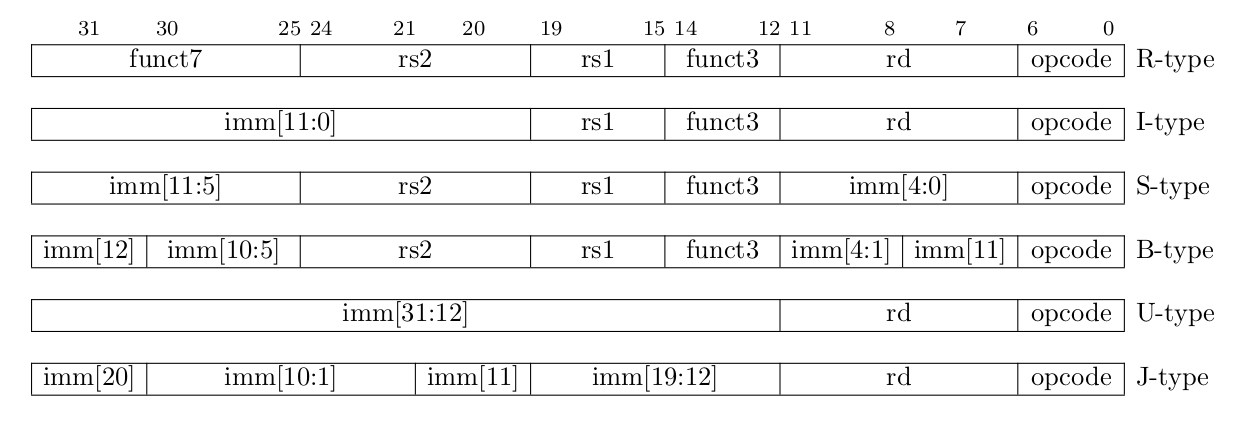
\includegraphics[width=0.7\textheight,keepaspectratio]{images/riscv_binary.png}
        \end{columns}
    \end{frame}
    
    \begin{frame}{\Romannum{2} генерација}
        \begin{columns}
            \column{0.38\linewidth}
            \begin{itemize}
                \item Инструкције су представљене својим симболичким називом
                \item Какво побољшање ово представља?
                \item Који недостаци су и даље присутни?
                \item Које типове уочавамо?
            \end{itemize}
            
            \column{0.58\linewidth}
            \centering
            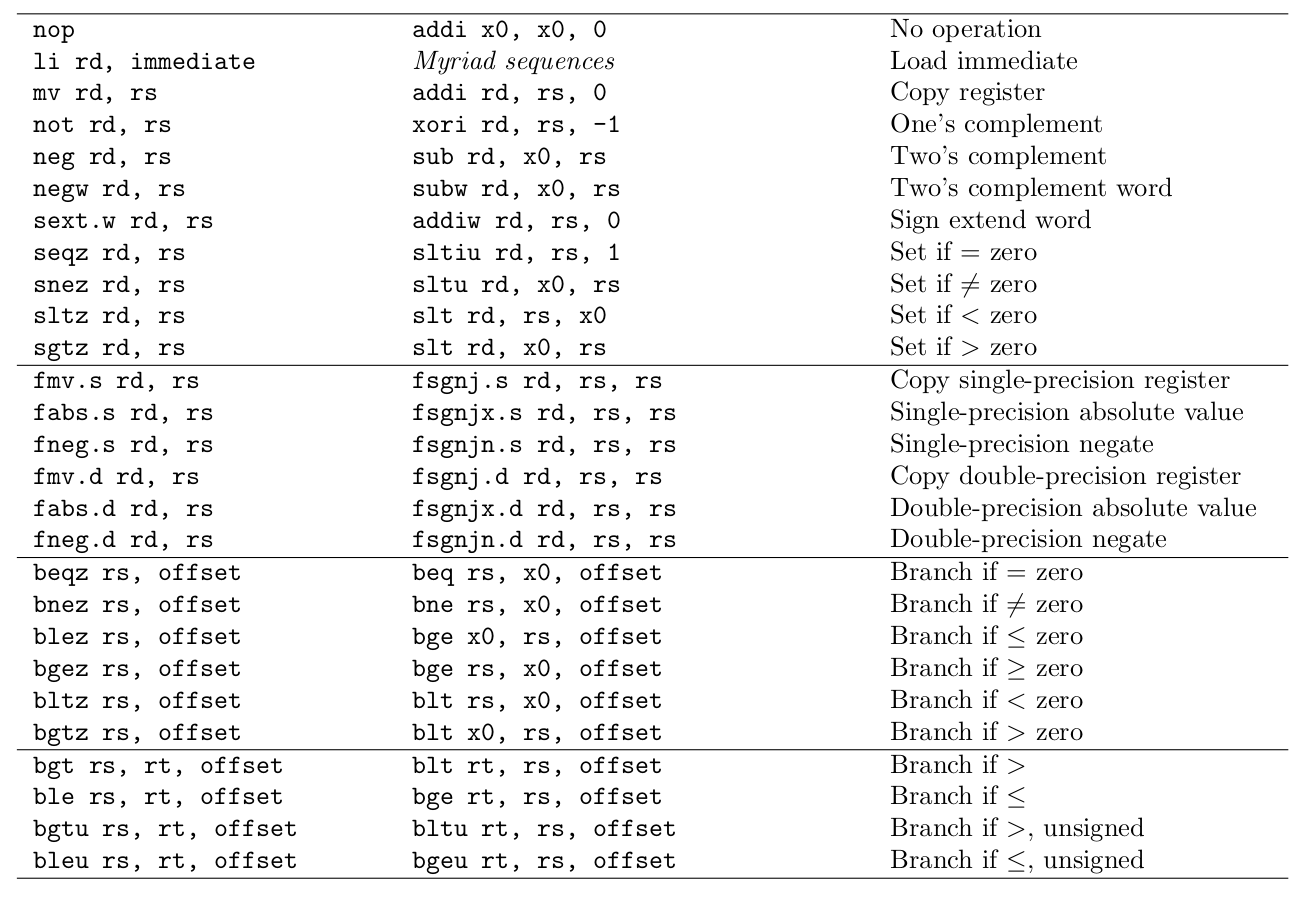
\includegraphics[width=0.7\textheight,keepaspectratio]{images/riscv_asm.png}
        \end{columns}
    \end{frame}
    
    \begin{frame}{\Romannum{3} генерација}
        \begin{columns}
            \column{0.38\linewidth}
            \begin{itemize}
                \item Структура програма слична стаблу
                \item Ограничен приступ меморији
                \item Ограничена слобода у условном гранању
                \item Подела на \textbf{исказе} и \textbf{изразе}
            \end{itemize}
            
            \column{0.58\linewidth}
            \centering
            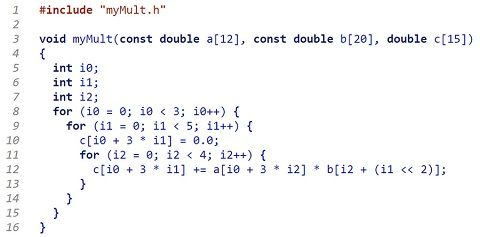
\includegraphics[width=0.7\textheight,keepaspectratio]{images/c.jpg}
        \end{columns}
    \end{frame}
    
    \begin{frame}{Теорија и пракса}
        \begin{columns}
            \column{0.48\linewidth}
            \begin{itemize}
                \item На најнижем нивоу апстракције, тип представља бинарни формат и правила за његово тумачење
                \item Ограничење је потребно како би се извршавао искључиво код који уме да интерпретира садржај на исправан начин
            \end{itemize}
            
            \column{0.48\linewidth}
            \begin{itemize}
                \item На вишем нивоу апстракције, тип представља скуп дозвољених вредности и дозвољених операција
                \item Ограничење је потребно како би се извршавале операције искључиво над семантички компатибилним ентитетима
            \end{itemize}
        \end{columns}
    \end{frame}
    
    \begin{frame}[allowframebreaks]{Мутабилност}
        \begin{itemize}
            \item Мутабилност је појам који постоји у рачунарству, али не постоји у математици
            \item Математика познаје само вредности
            \item Вредности могу да припадају скуповима и променљиве могу да имају одређену вредност
            \item Вредности које припадају скупу су унапред задате дефиницијом скупа
            \item Међутим, природа \textbf{променљивости} саме вредности није дефинисана!
            \item Сматра се да је сама вредност \textbf{целовита} и \textbf{непроменљива}, док је могуће да променљива има различите вредности!
        \end{itemize}
        
        \framebreak
        
        \begin{itemize}
            \item Рачунарство такође познаје појам променљиве и вредности, али уводи и једно својство које сведочи о променљивости саме вредности
            \item Речником рачунарства, вредности у математици су имутабилне
            \item Више променљивих може да показује на исту вредност (показивачи), због чега измена саме вредности постаје видљива преко различитих променљивих!
            \item У рачунарству постоји ограничење задато хардвером (и у крајњој граници, законима физике) које захтева увођење оваквог својства
        \end{itemize}
        
        \framebreak
        
        \begin{itemize}
            \item Прости типови заузимају мало простора, због чега је њихово складиштење на стеку и у регистрима једноставно
            \item Креирање копија вредности простих типова је једноставно и брзо
            \item Сложени типови заузимају далеко више простора и најчешће се складиште на хипу
            \item Стање мутабилних објеката је могуће мењати и након креирања
            \item Мутабилност побољшава перформансе, али уноси непредвидивост
            \begin{itemize}
                \item имате ли идеју како?
            \end{itemize}
            \item Мутабилност утиче на дизајн система типова!
            \begin{itemize}
                \item више речи о овоме нешто касније
            \end{itemize}
        \end{itemize}
    \end{frame}
    
    \begin{frame}{Мутабилни објекти}
        \begin{figure}
            \centering
            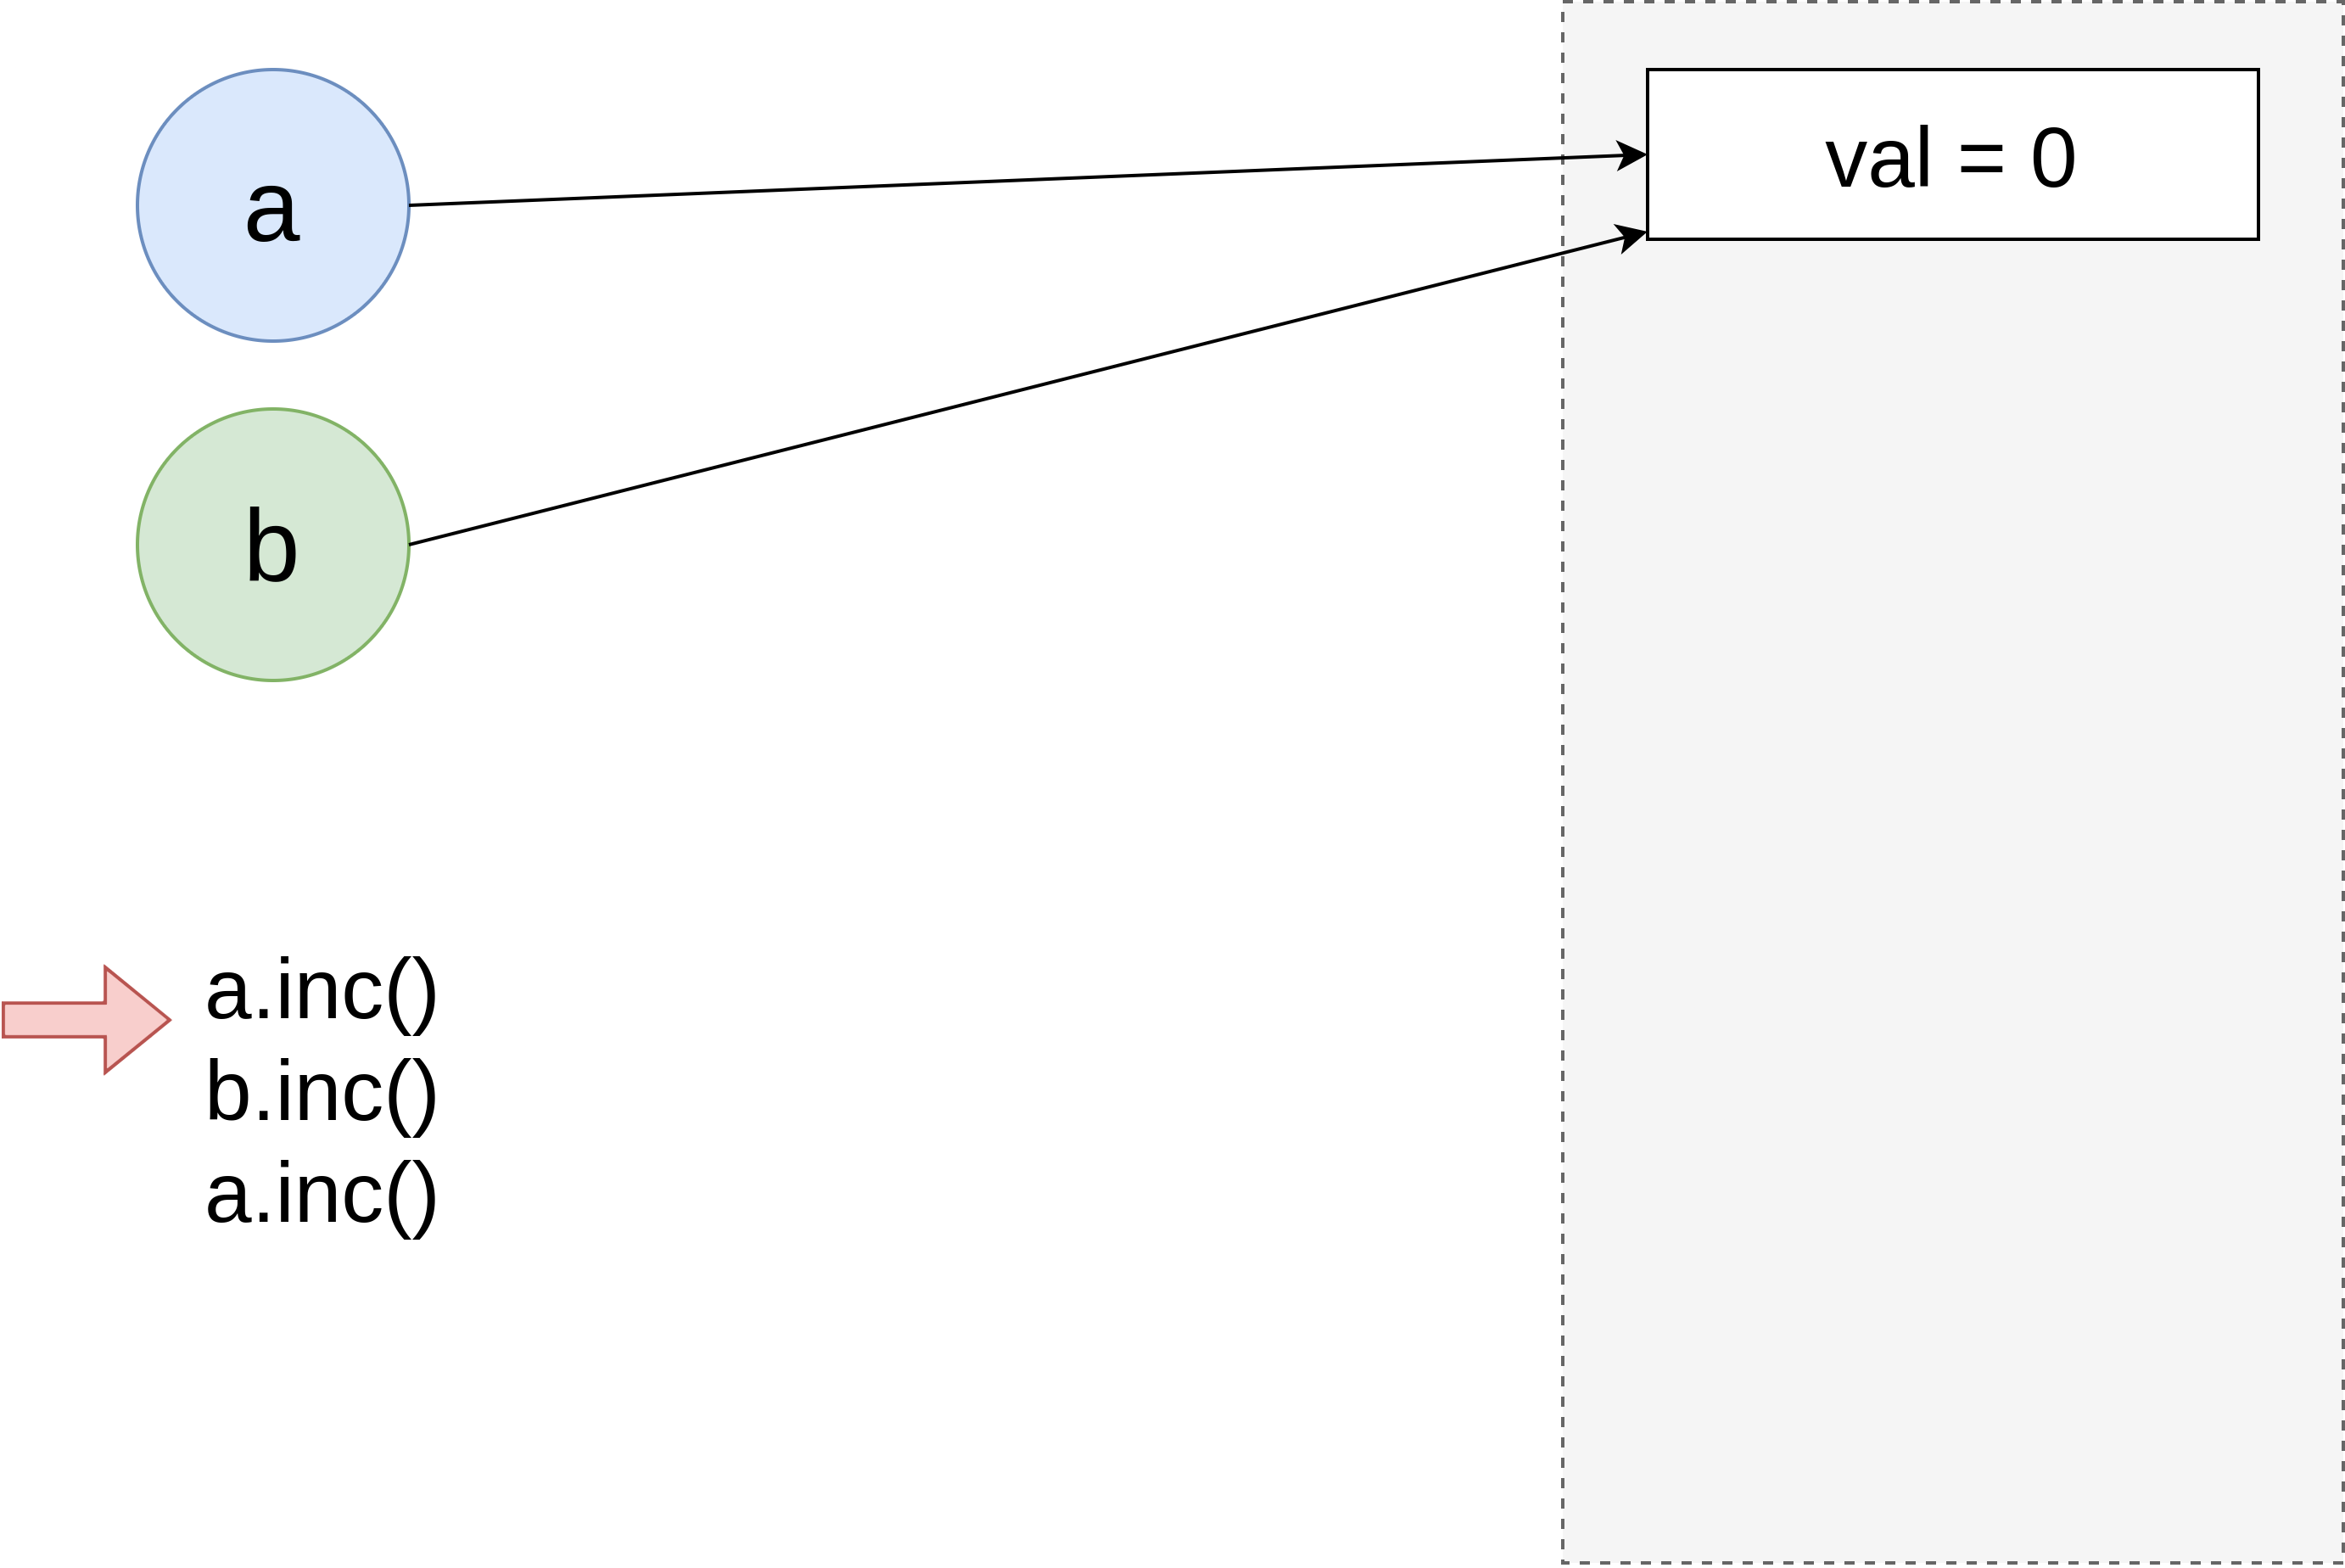
\includegraphics[height=0.7\textheight,keepaspectratio]{images/mut0.png}
        \end{figure}
    \end{frame}
    
    \begin{frame}{Мутабилни објекти}
        \begin{figure}
            \centering
            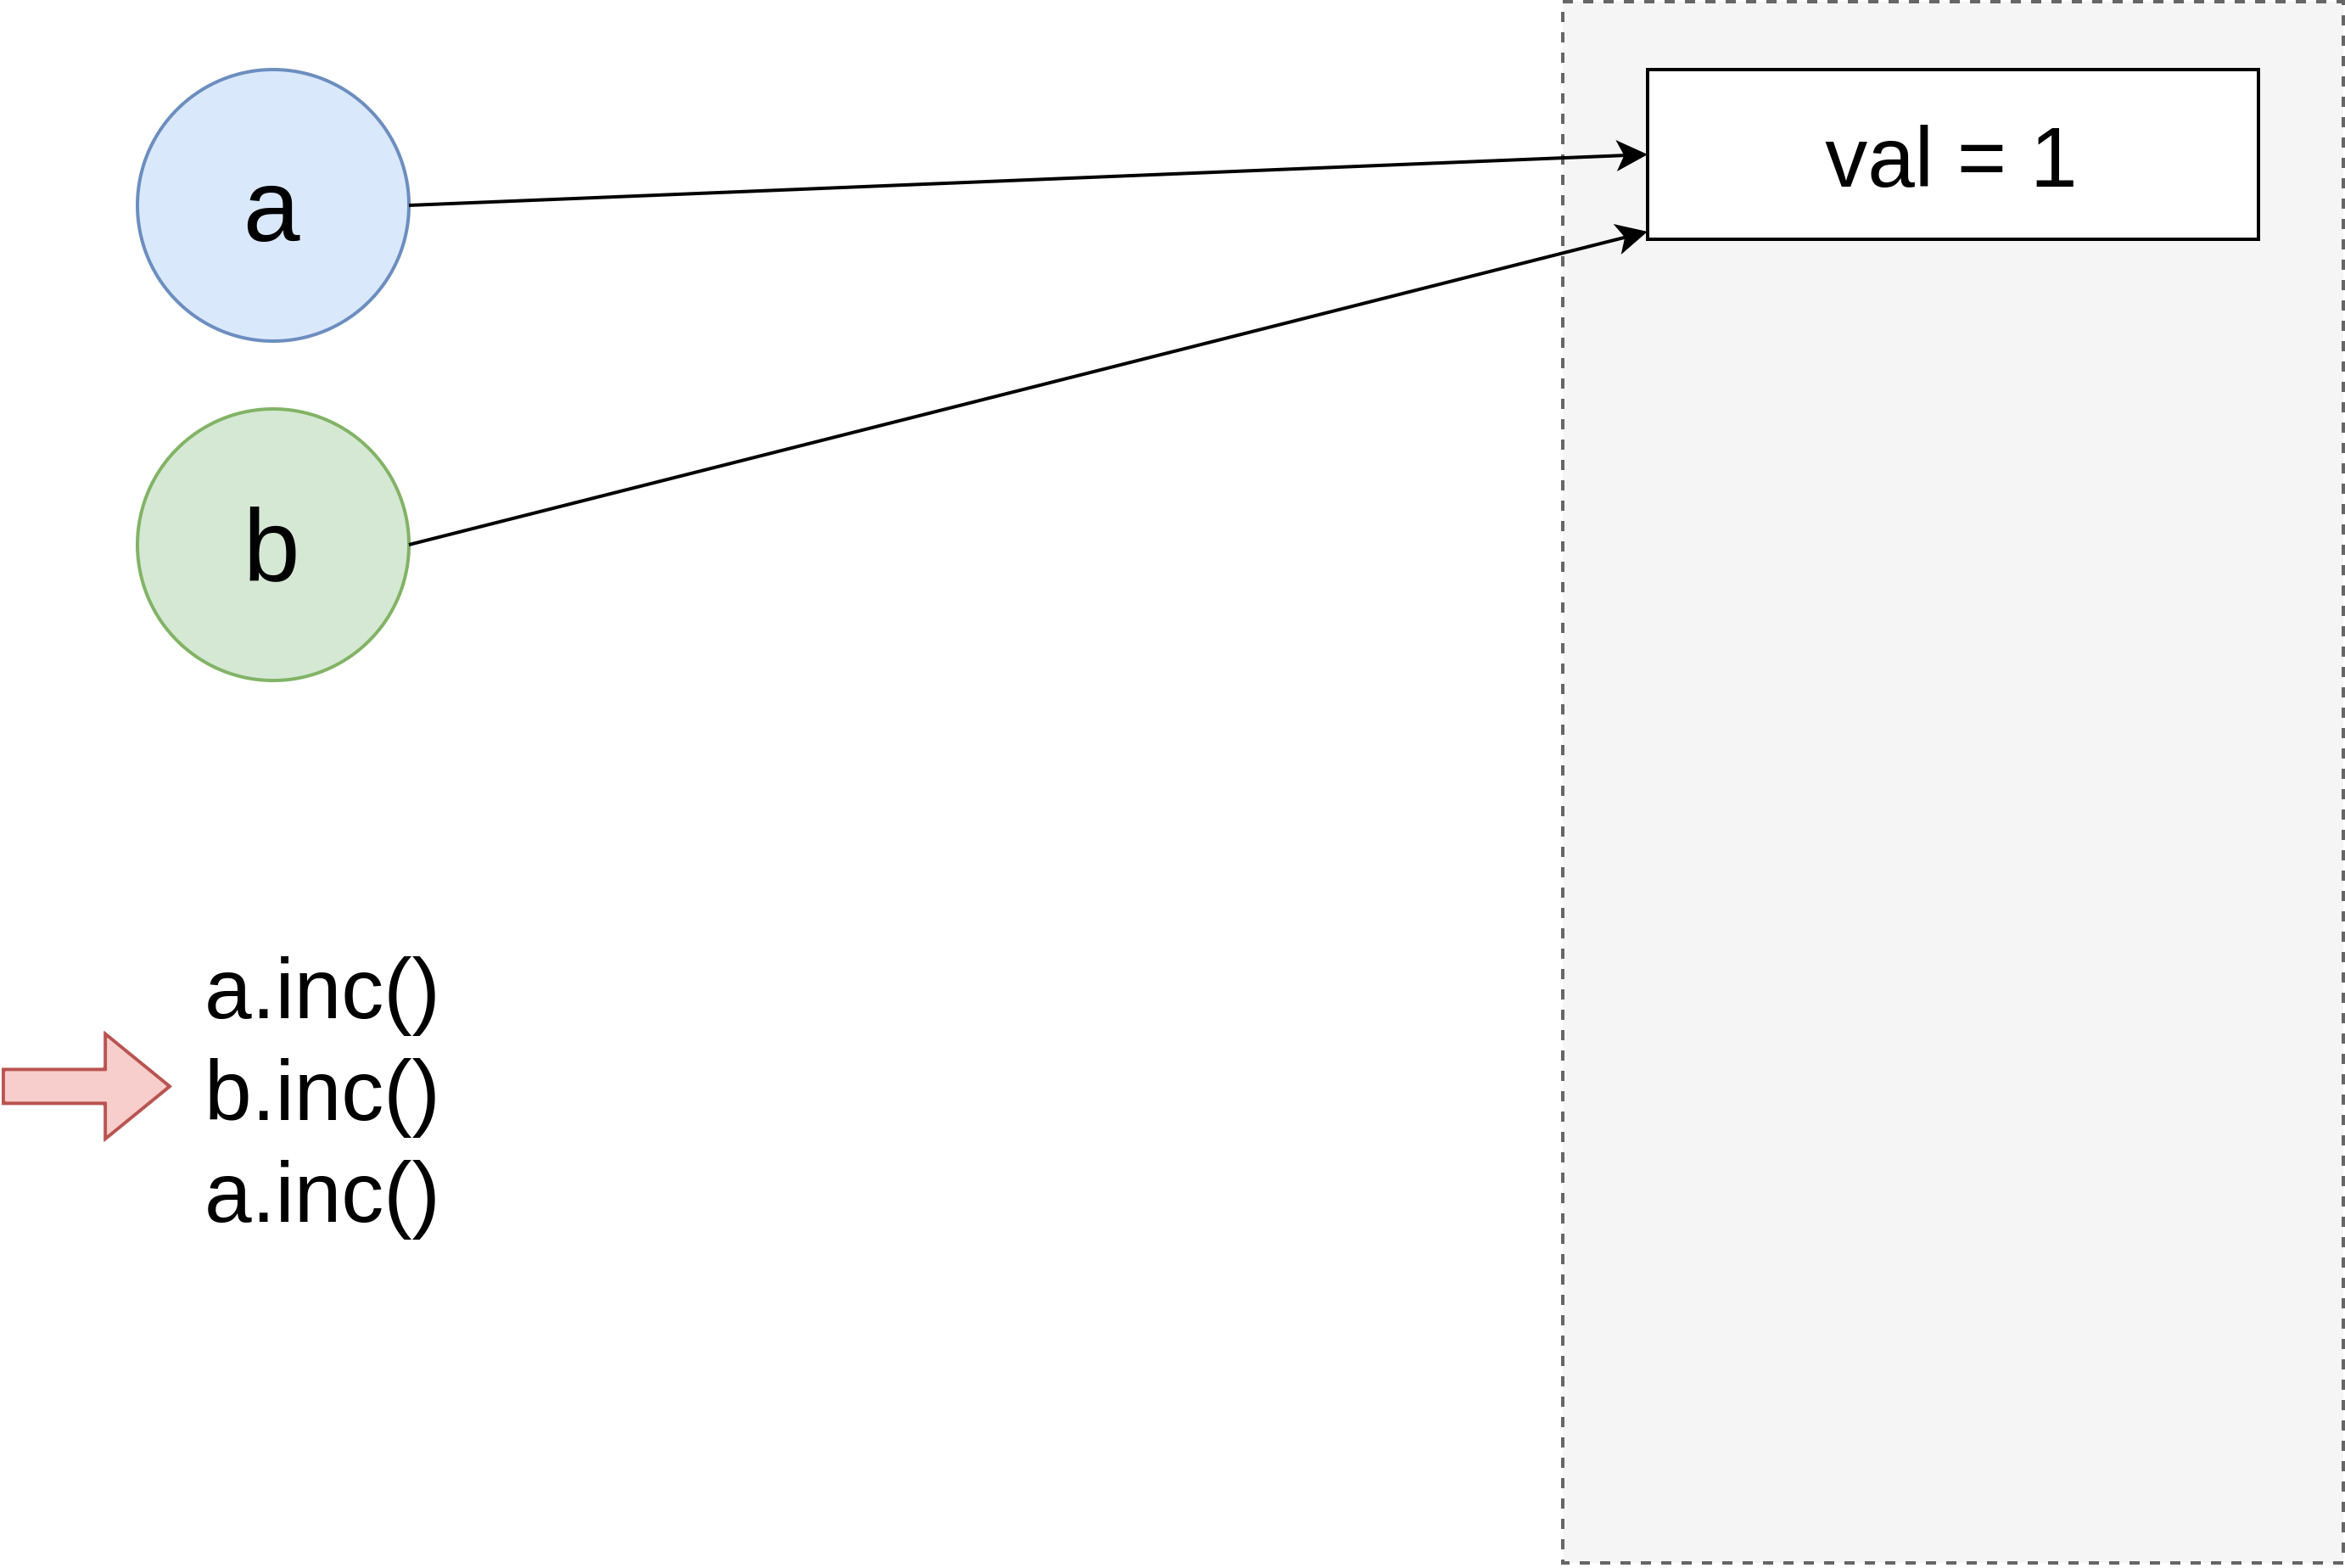
\includegraphics[height=0.7\textheight,keepaspectratio]{images/mut1.png}
        \end{figure}
    \end{frame}
    
    \begin{frame}{Мутабилни објекти}
        \begin{figure}
            \centering
            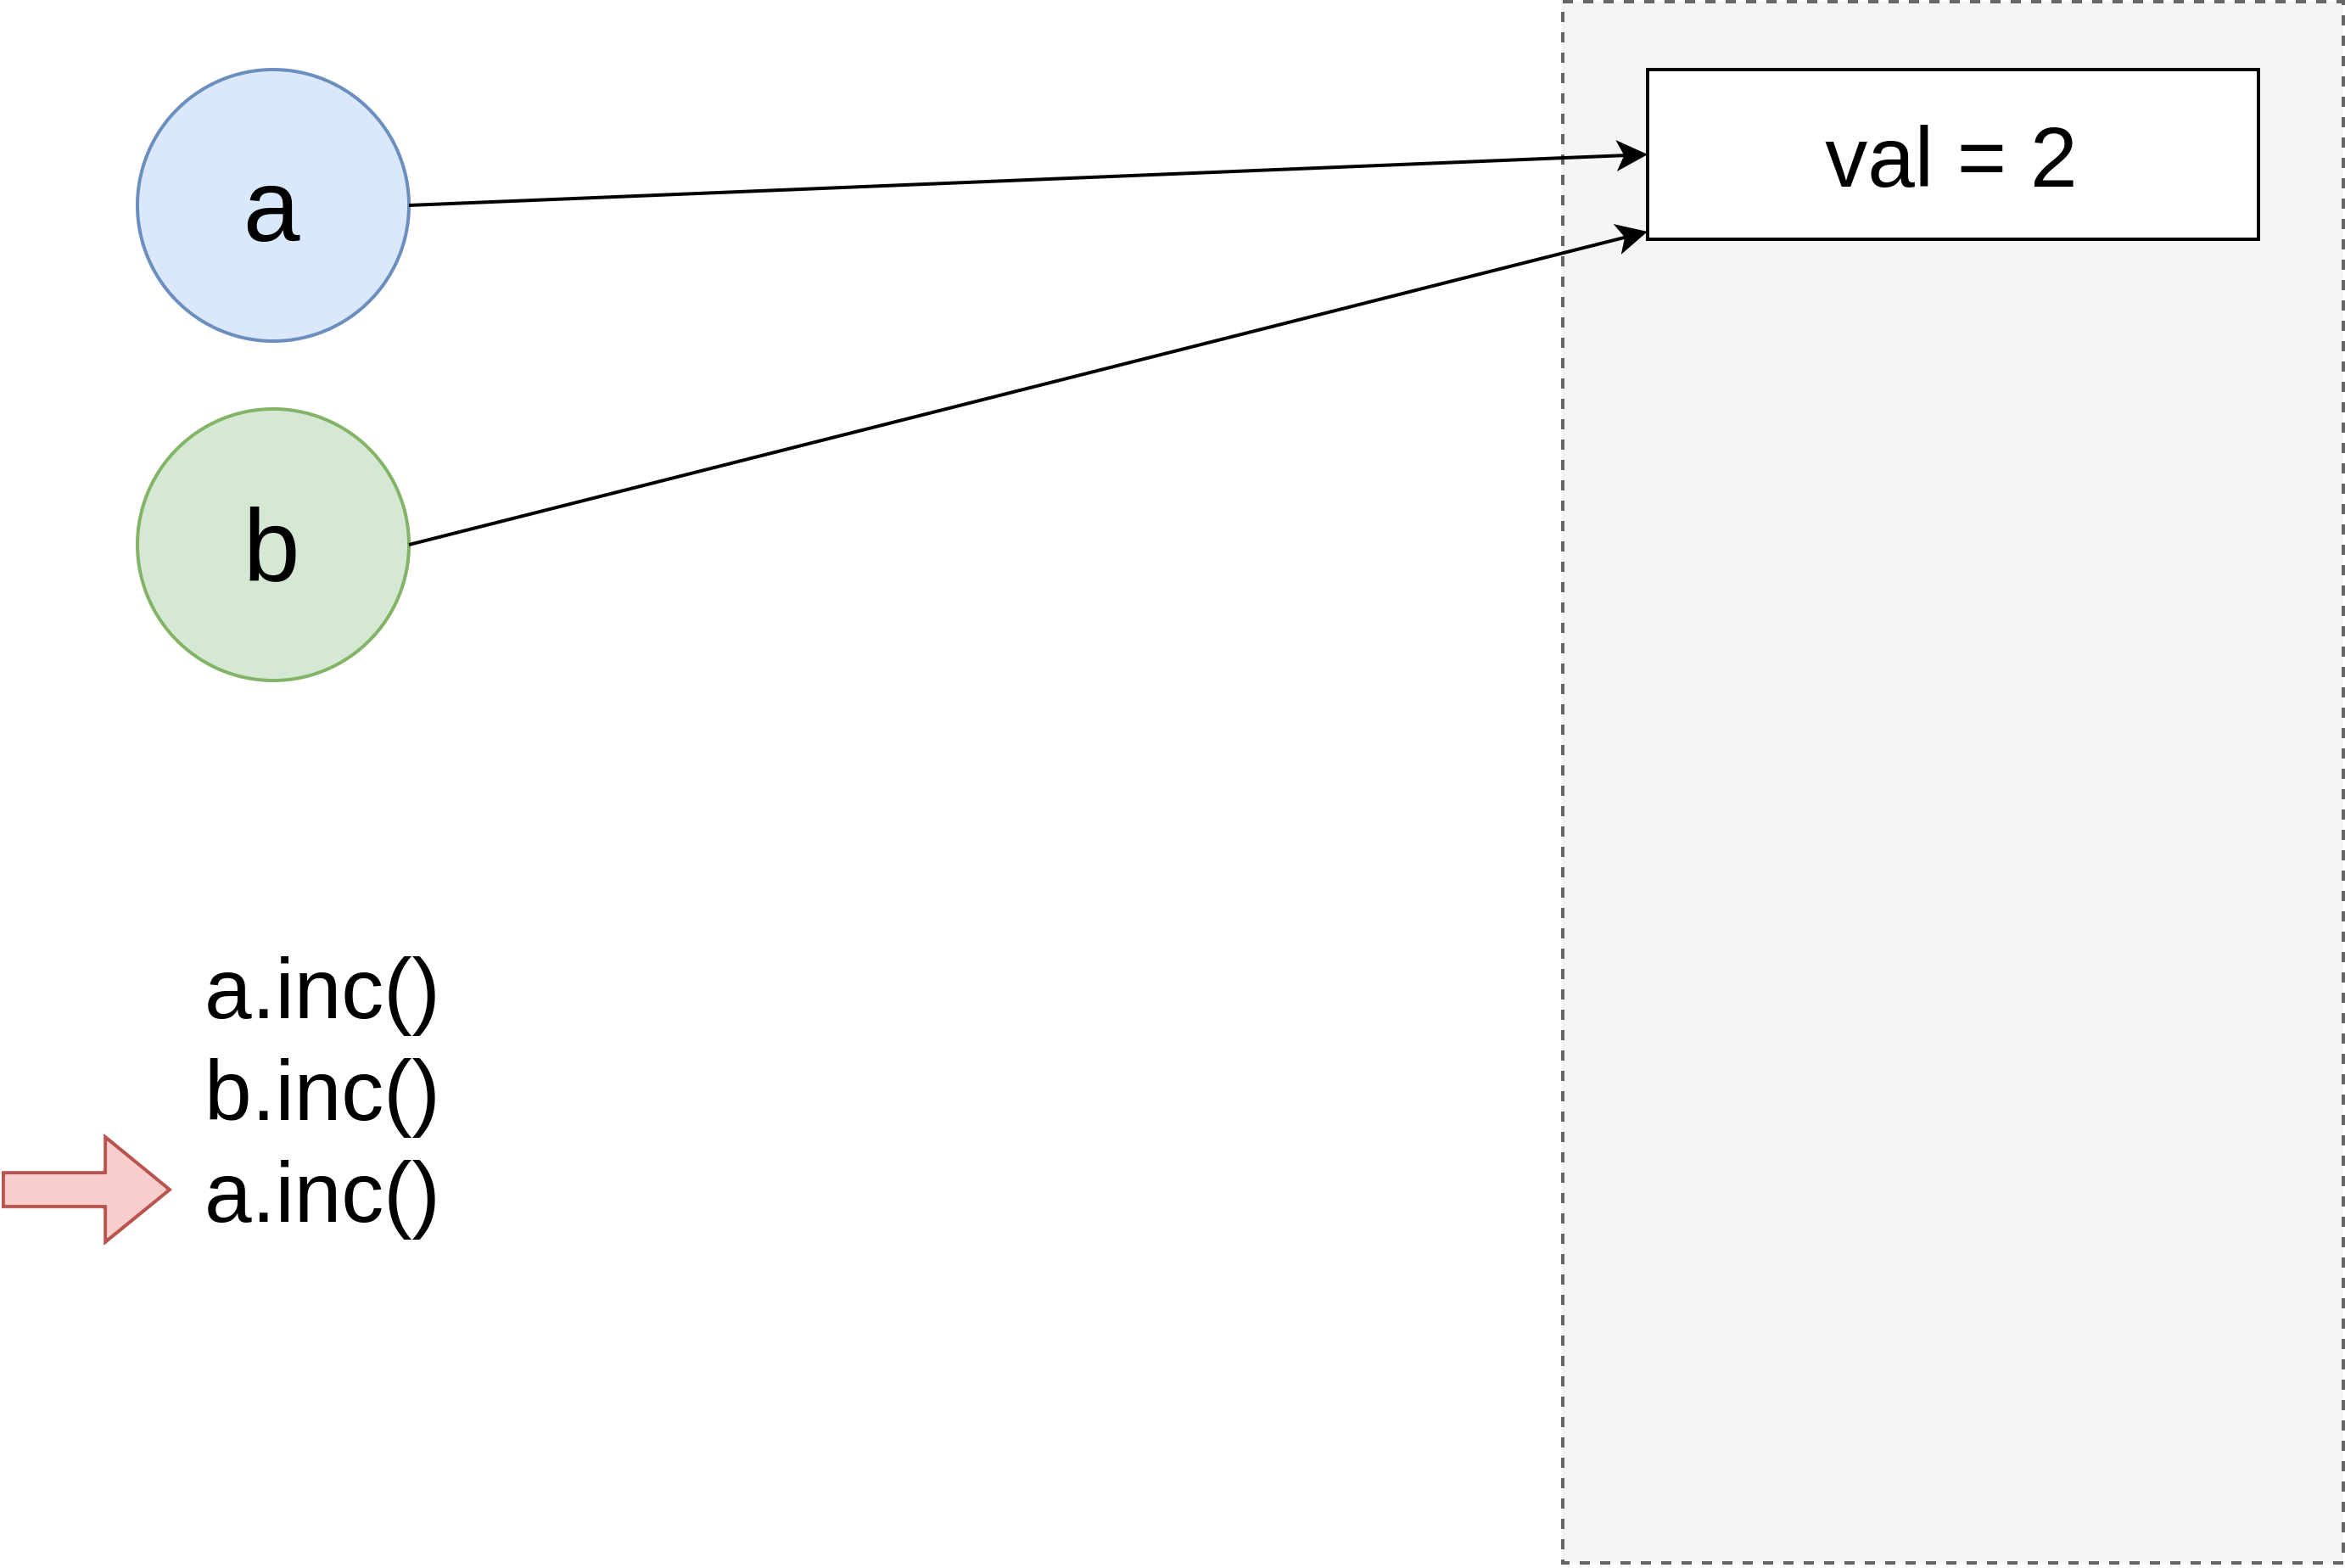
\includegraphics[height=0.7\textheight,keepaspectratio]{images/mut2.png}
        \end{figure}
    \end{frame}
    
    \begin{frame}{Имутабилни објекти}
        \begin{figure}
            \centering
            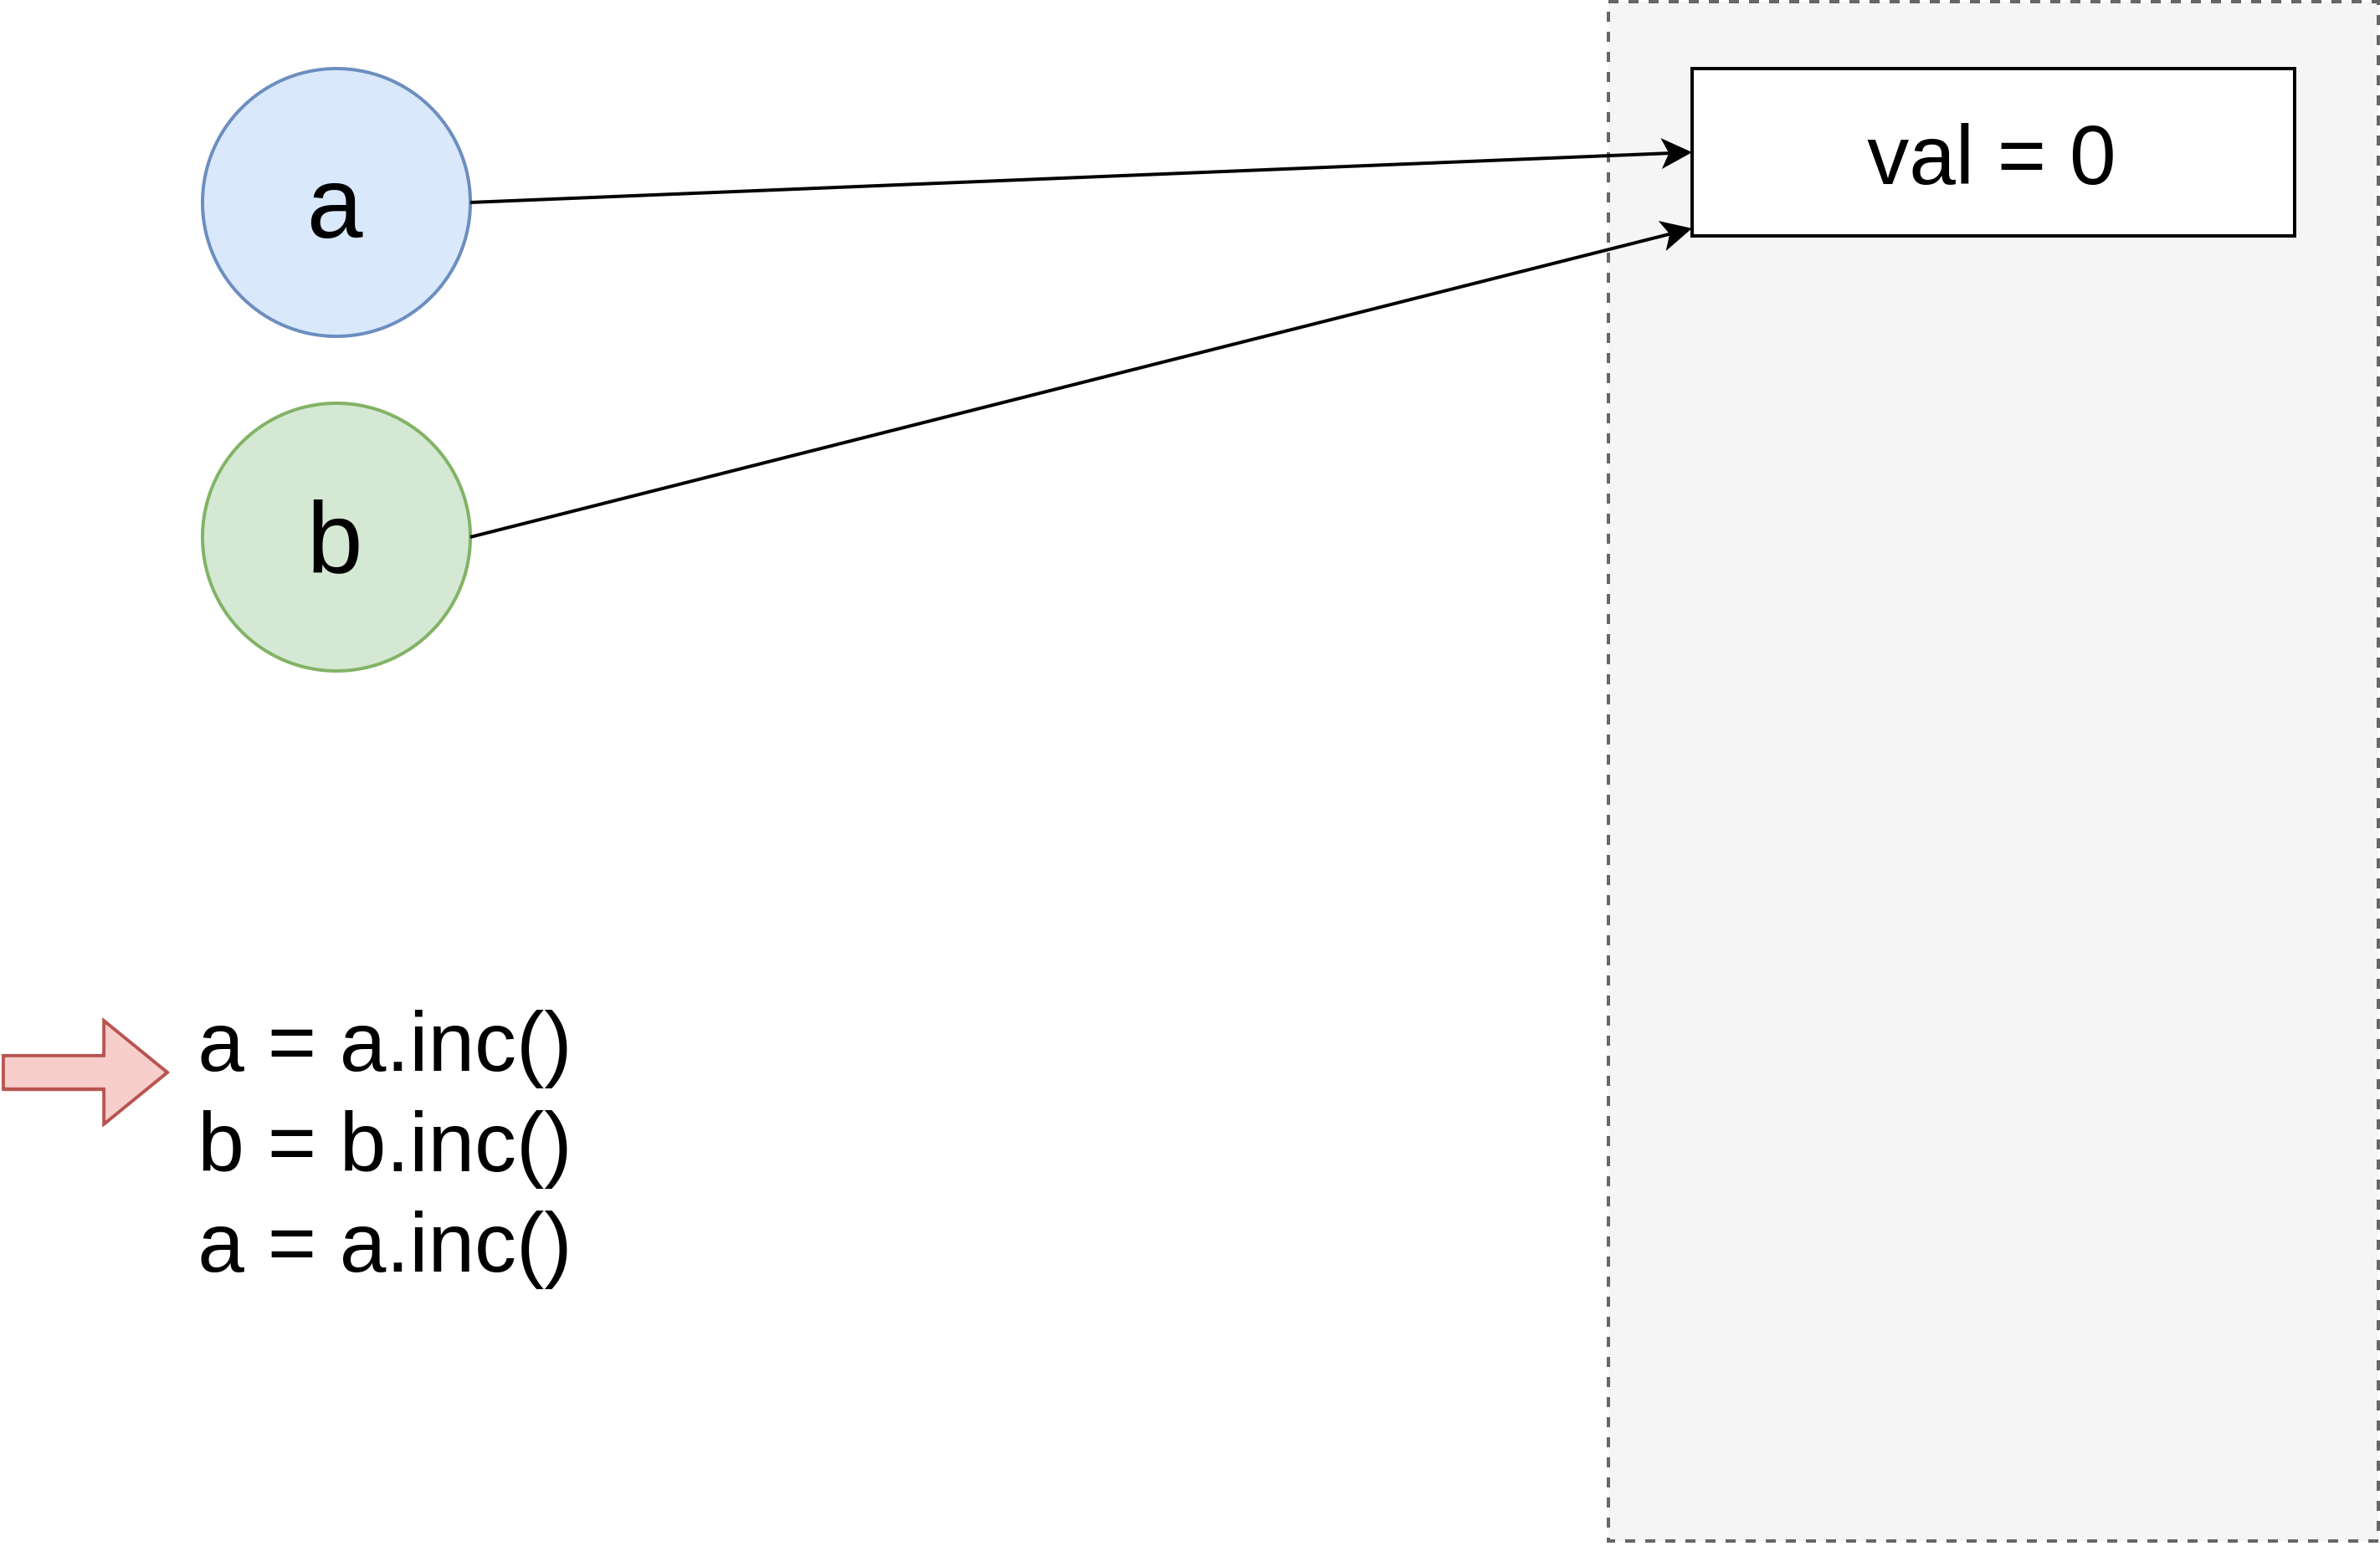
\includegraphics[height=0.7\textheight,keepaspectratio]{images/imut0.png}
        \end{figure}
    \end{frame}
    
    \begin{frame}{Имутабилни објекти}
        \begin{figure}
            \centering
            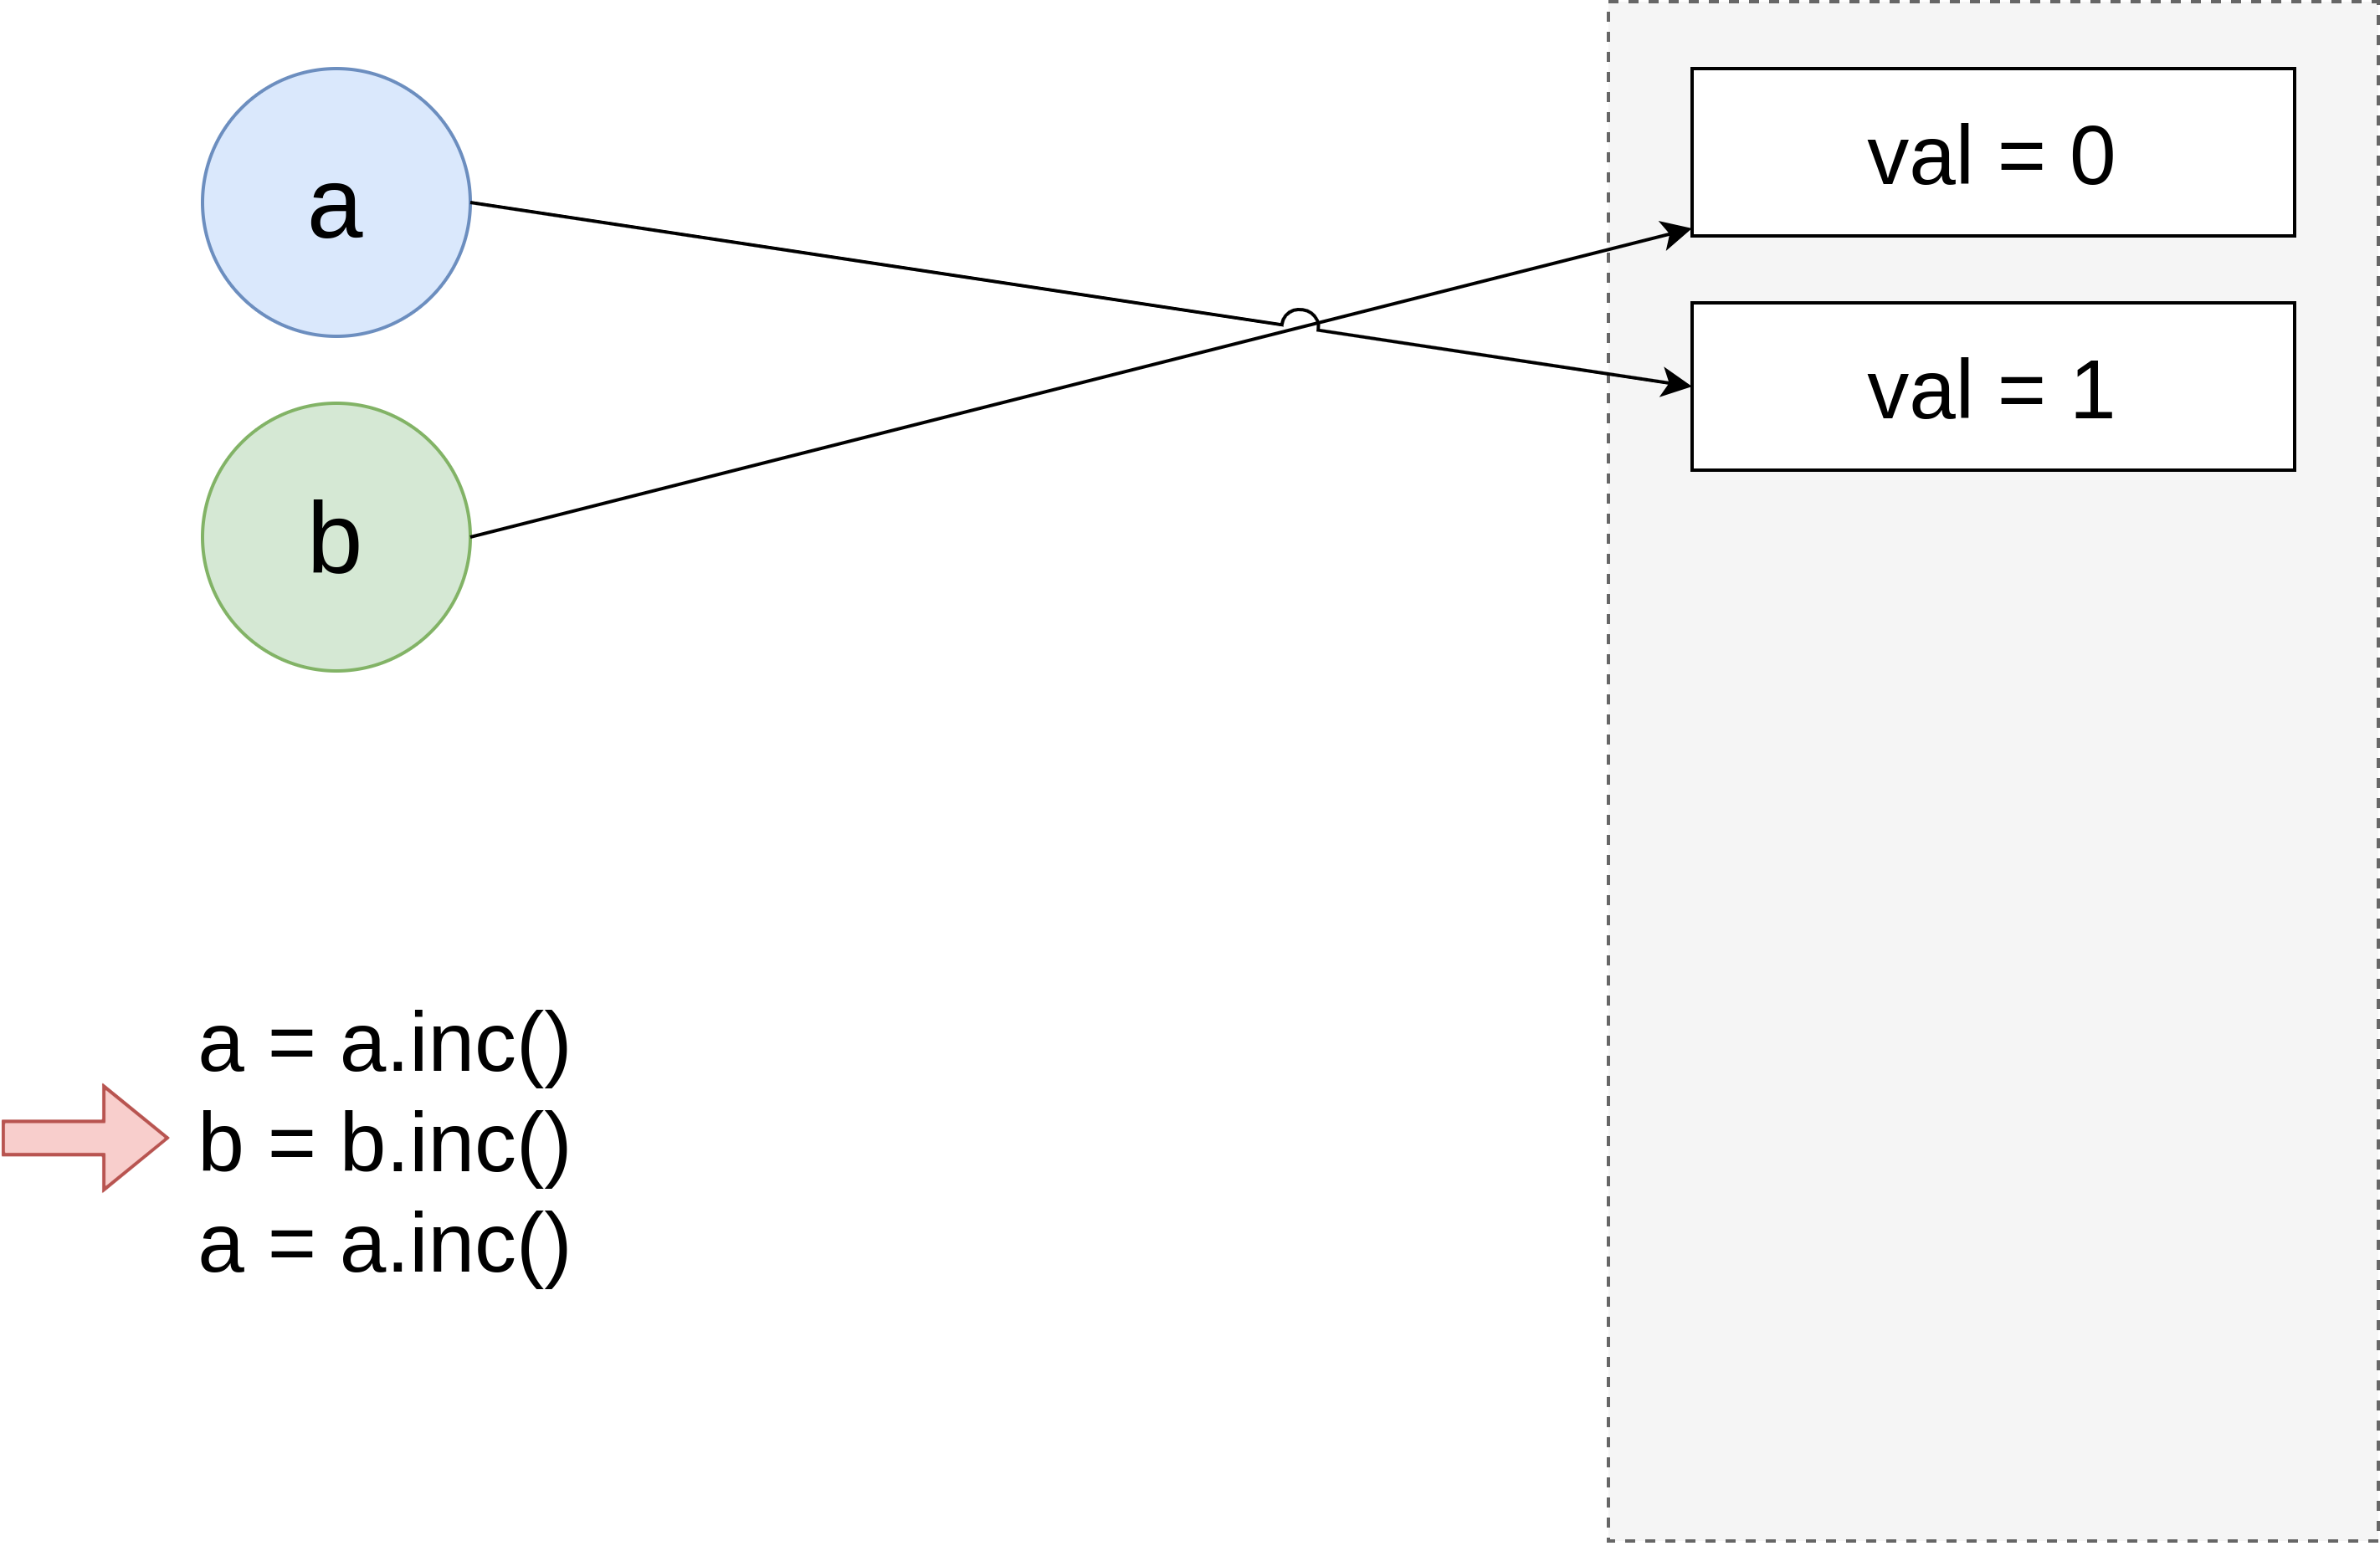
\includegraphics[height=0.7\textheight,keepaspectratio]{images/imut1.png}
        \end{figure}
    \end{frame}
    
    \begin{frame}{Имутабилни објекти}
        \begin{figure}
            \centering
            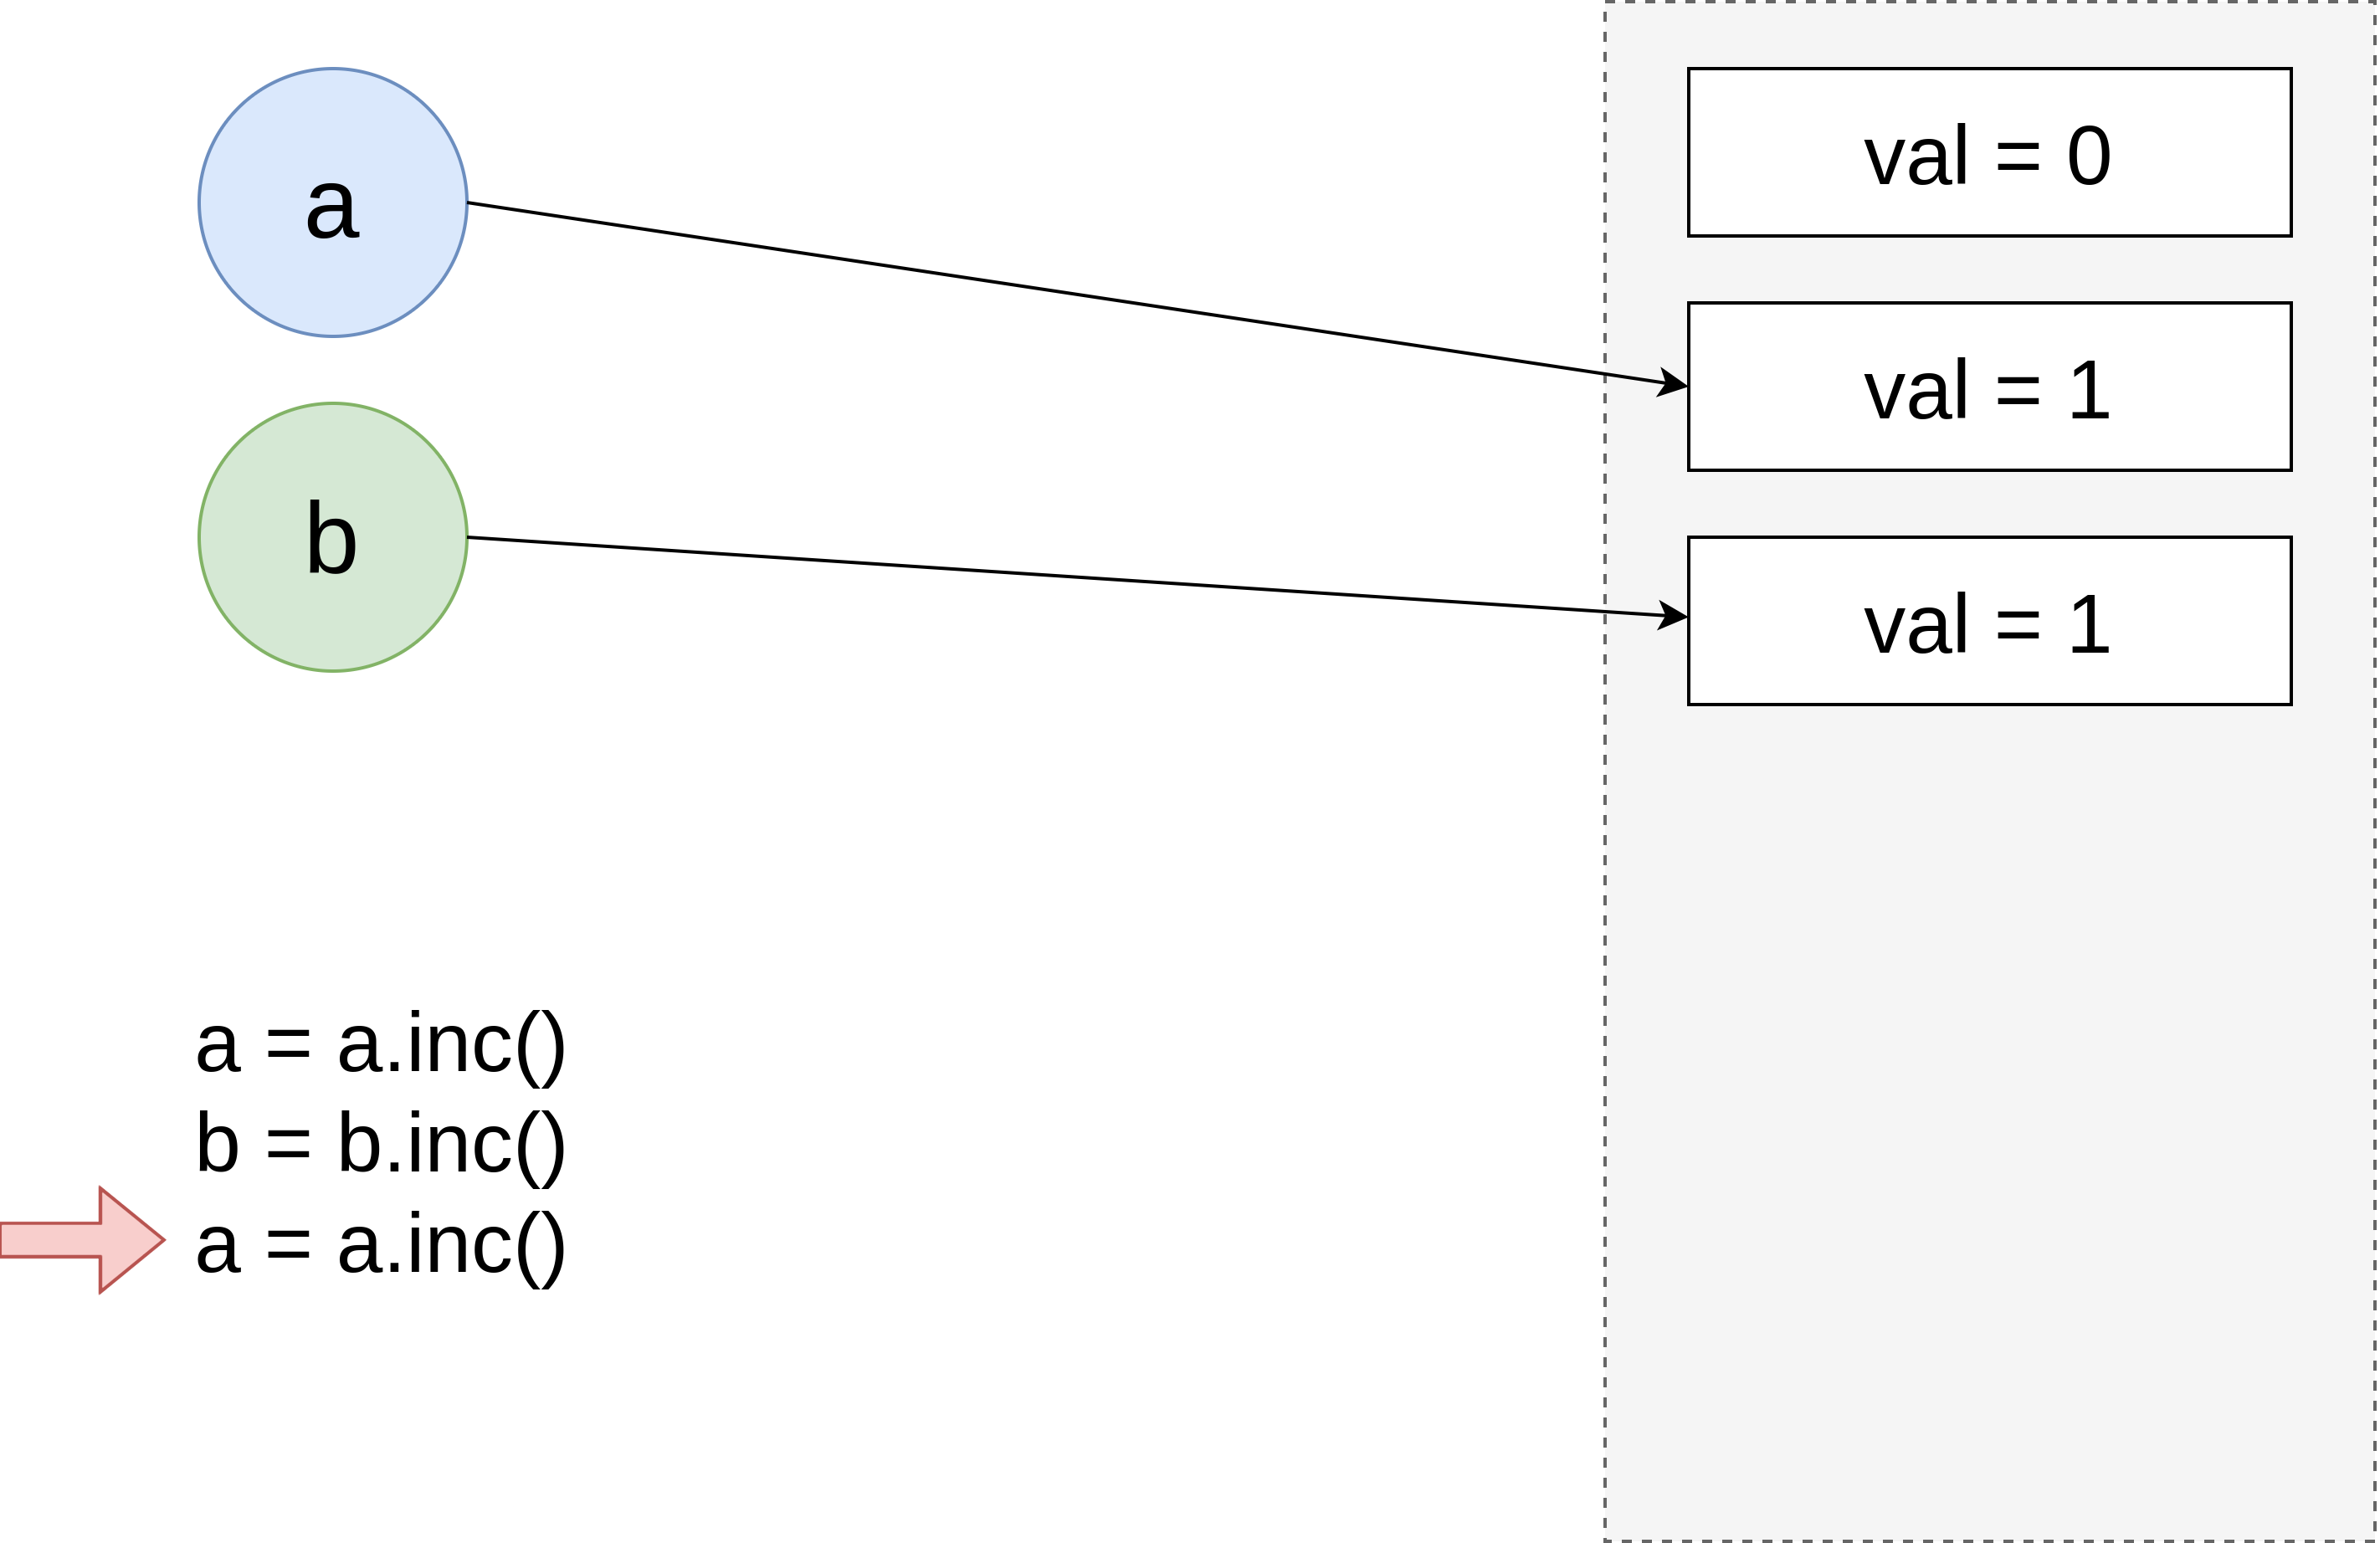
\includegraphics[height=0.7\textheight,keepaspectratio]{images/imut2.png}
        \end{figure}
    \end{frame}

    \begin{frame}{Теорија типова и теорија скупова}
        \begin{itemize}
            \item Једнакост типова осигурава исправност програма
            \item Да ли отежава писање програма?
            \begin{itemize}
                \item у стварном свету, уочавамо сличност између различитих појмова и облика
                \item некада су ти појмови довољно слични да можемо да занемаримо разлике
                \item пример: потребан нам је аутомобил, али нас не занима произвођач
            \end{itemize}
            \item Тип је појам сродан скупу
            \item Ако постоје подскупови, да ли постоје и подтипови?
            \item Шта описују подскупови, а шта би описивали подтипови?
            \item Релација подтипа је слична релацији подскупа!
        \end{itemize}
    \end{frame}
    
    \begin{frame}{Конвертибилност типова (релација подтипа)}
        \begin{itemize}
            \item Кажемо да је \begin{math}A \leq B\end{math} уколико је \begin{math}A\end{math} конвертибилно у \begin{math}B\end{math}
            \begin{itemize}
                \item \begin{math}A \leq B\end{math} \textbf{(рефлексивност)}
                \item \begin{math}A \leq B \wedge B \leq C \Rightarrow A \leq C\end{math} \textbf{(транзитивност)}
                \item \begin{math}A \leq B \wedge B \leq A \Rightarrow A = B\end{math} \textbf{(антисиметричност)}
            \end{itemize}
            \item Релација подтипа је релација парцијалног поретка!
        \end{itemize}
    \end{frame}

    \begin{frame}[allowframebreaks]{Шта одређује конвертибилност типова?}
        \begin{itemize}
            \item Правила која дефинишу конвертибилност типова су одлука дизајнера система типова
            \item Главни водич је тип А мора да садржи све вредности које подржава Б као и да приликом имплицитне конверзије не долази до губитка података
            \begin{itemize}
                \item Релативан појам: скуп целих бројева је подскуп скупа реалних бројева у математици, док је у програмирању могућ губитак приликом претварања целобројне вредности у вредност са покретним зарезом
                \item Неки програмски језици ово игноришу, док други ово сматрају за грешку и захтевају експлицитну конверзију целобројног типа
            \end{itemize}
            \item Додатно: мутабилност не сме да изазове грешке приликом извршавања програма
        \end{itemize}
        
        \framebreak
        
        \begin{itemize}
            \item За просте типове, конвертибилност је дефинисана правилима система типова
            \item За сложене типове, конвертибилност је релацијом између сложених типова (коју задаје корисник) и/или у односу на садржај (правила дефинише систем типова)
            \begin{itemize}
                \item више речи о овоме нешто касније
            \end{itemize}
        \end{itemize}
    \end{frame}

    \begin{frame}{Закључивање типова}
        \begin{itemize}
            \item До сада смо разумели појам типа, система типова и релације подтипа
            \item Како можемо да стечено знање употребимо за решавање полазног проблема: одређивање исправности израза?
            \item Као и сваки формални систем, и систем типова се састоји од аксиома и правила
            \item Идеја: типови простих израза (литерали и променљиве) су познати (аксиоми), а тип сложеног израза је могуће закључити уколико су подизрази одговарајућих типова (правила)
        \end{itemize}
    \end{frame}

    \begin{frame}{Правила}
        \begin{itemize}
            \item Бинарни изрази:
            \begin{itemize}
                \item оба подизраза морају да имају заједнички тип у који су конвертибилни како би операција била могућа
                \item резултат бинарне аритметичке операције је заједничког типа
                \item резултат бинарне логичке или релацине операције је булова вредсноти
            \end{itemize}
            \item Позив функције:
            \begin{itemize}
                \item евалуација позива функције враћа вредност типа повратног типа функције
                \item шта је још потребно да би позив био могућ?
            \end{itemize}
        \end{itemize}
    \end{frame}

    \begin{frame}{Сложени типови}
        \begin{itemize}
            \item До сада смо разумели просте типове као и њихову примену
            \item Уочавамо потребу за креирањем сложених типова
            \begin{itemize}
                \item једноставан пример: желимо обраду над скупом простих типова
                \item напреднији пример: желимо да ентитете из стварног света представимо у програмима, уз задржавање правила за аутоматску проверу исправности
                \item додатно: постоји потреба да ентитете програмског језика (попут фунцкија) опишемо типом, како би могли да их обрађујемо на исти начин као и корисничке типове
            \end{itemize}
            \item Како бисмо могли да креирамо овакве типове?
        \end{itemize}
    \end{frame}

    \begin{frame}{Конструктор типа}
        \begin{itemize}
            \item Конструктор типа омогућава креирање новог типа користећи претходно дефинисане типове
            \item Подсетник: систем типова дефинише основне типове
            \item Додатно: систем типова дефинише конструкторе типова
            \item Омогућено је произвољно комбиновање типова без обзира на контекст
            \begin{itemize}
                \item аксиоми и правила система типова омогућавају проверу исправности употребе у односу на релацију подтипа
            \end{itemize}
        \end{itemize}
    \end{frame}

    \begin{frame}[allowframebreaks]{Низови}
        \begin{itemize}
            \item Низови су најједноставнији пример сложеног типа
            \item У пракси, честа је потреба за обрадом колекције података
            \item Желимо да спречимо складиштење произвољних вредности како би омогућили униформну обраду
            \item Да ли је услов за униформну обраду једнакост типова () или релација подтипа ()?
            \item Можемо ли да упоредимо два типа низова?
        \end{itemize}

        \framebreak

        \begin{itemize}
            \item У низ Т[] можемо да ускладиштимо вредност x: X уколико X <= T
            \begin{itemize}
                \item T представља горњу границу типа вредности у низу!
            \end{itemize}
            \item У променљиву y: A[] можемо да ускладиштимо низ x: B[] уколико је B <= A
            \begin{itemize}
                \item тип низа је коваријантан у односу на тип Т
                \item да ли морамо да водимо рачуна и о дужини низа?
            \end{itemize}
        \end{itemize}
    \end{frame}

    \begin{frame}{Коваријантност типова}
        \textit{Сложени тип \begin{math}{A\mathord{<}T\mathord{>}}\end{math} је коваријантан у односу на тип параметра \begin{math}T\end{math} уколико важи \begin{math}{A\mathord{<}X\mathord{>} \leq A\mathord{<}Y\mathord{>}}\end{math} за \begin{math}X \leq Y\end{math}}
    \end{frame}
    
    \begin{frame}[allowframebreaks]{Варијантност и мутабилност}
        \begin{itemize}
            \item Имутабилни низови су очигледно коваријантни у односу на Т
            \item Проблем: шта се дешава уколико су низови мутабилни?
        \end{itemize}
        
        \framebreak
        
        \begin{math}
        A \leq B \leq C
\newline
\newline
a: A[] = [A, A, A]
\newline
b: B[] = a
\newline
\newline
b.add(B)
\newline
\newline
\text{Грешка: није могуће сачувати вредност} \newline B\space \text{у објекту типa} A \text{јер не важи} B \leq A\text{!}
        \end{math}
        
        \framebreak
        
        \begin{figure}
            \centering
            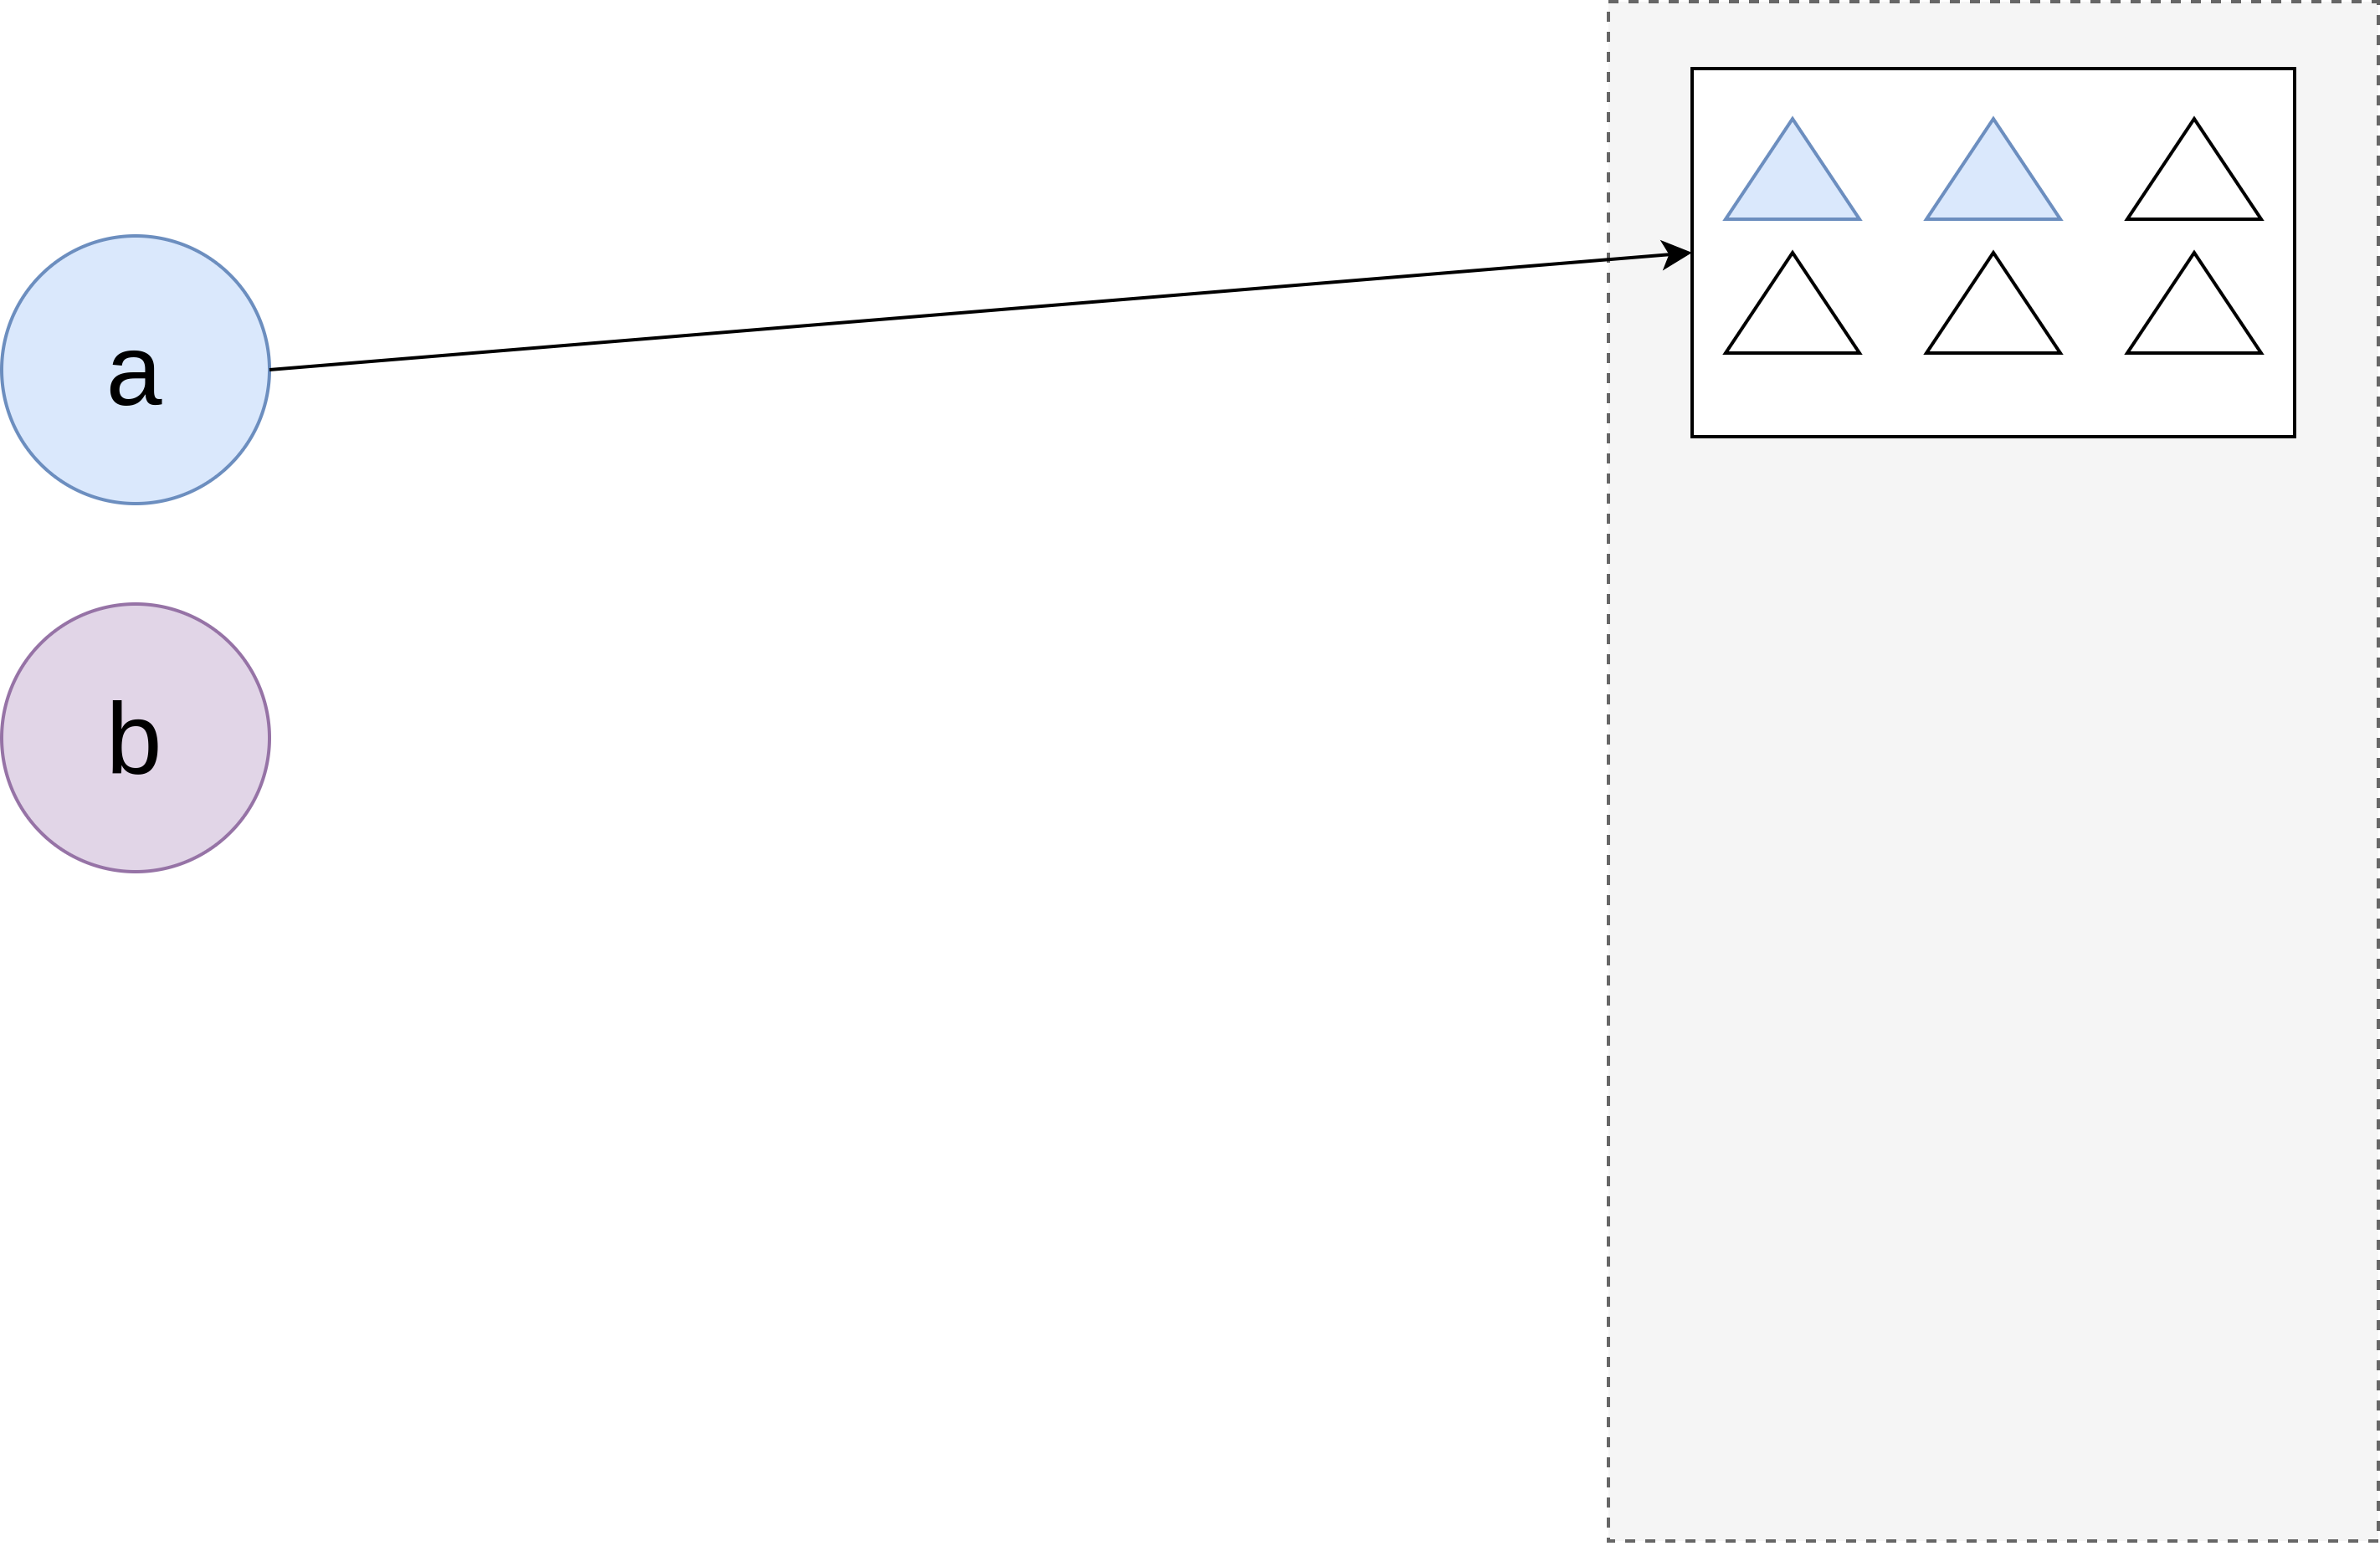
\includegraphics[height=0.7\textheight,keepaspectratio]{images/arr0.png}
        \end{figure}
        
        \framebreak
        
        \begin{figure}
            \centering
            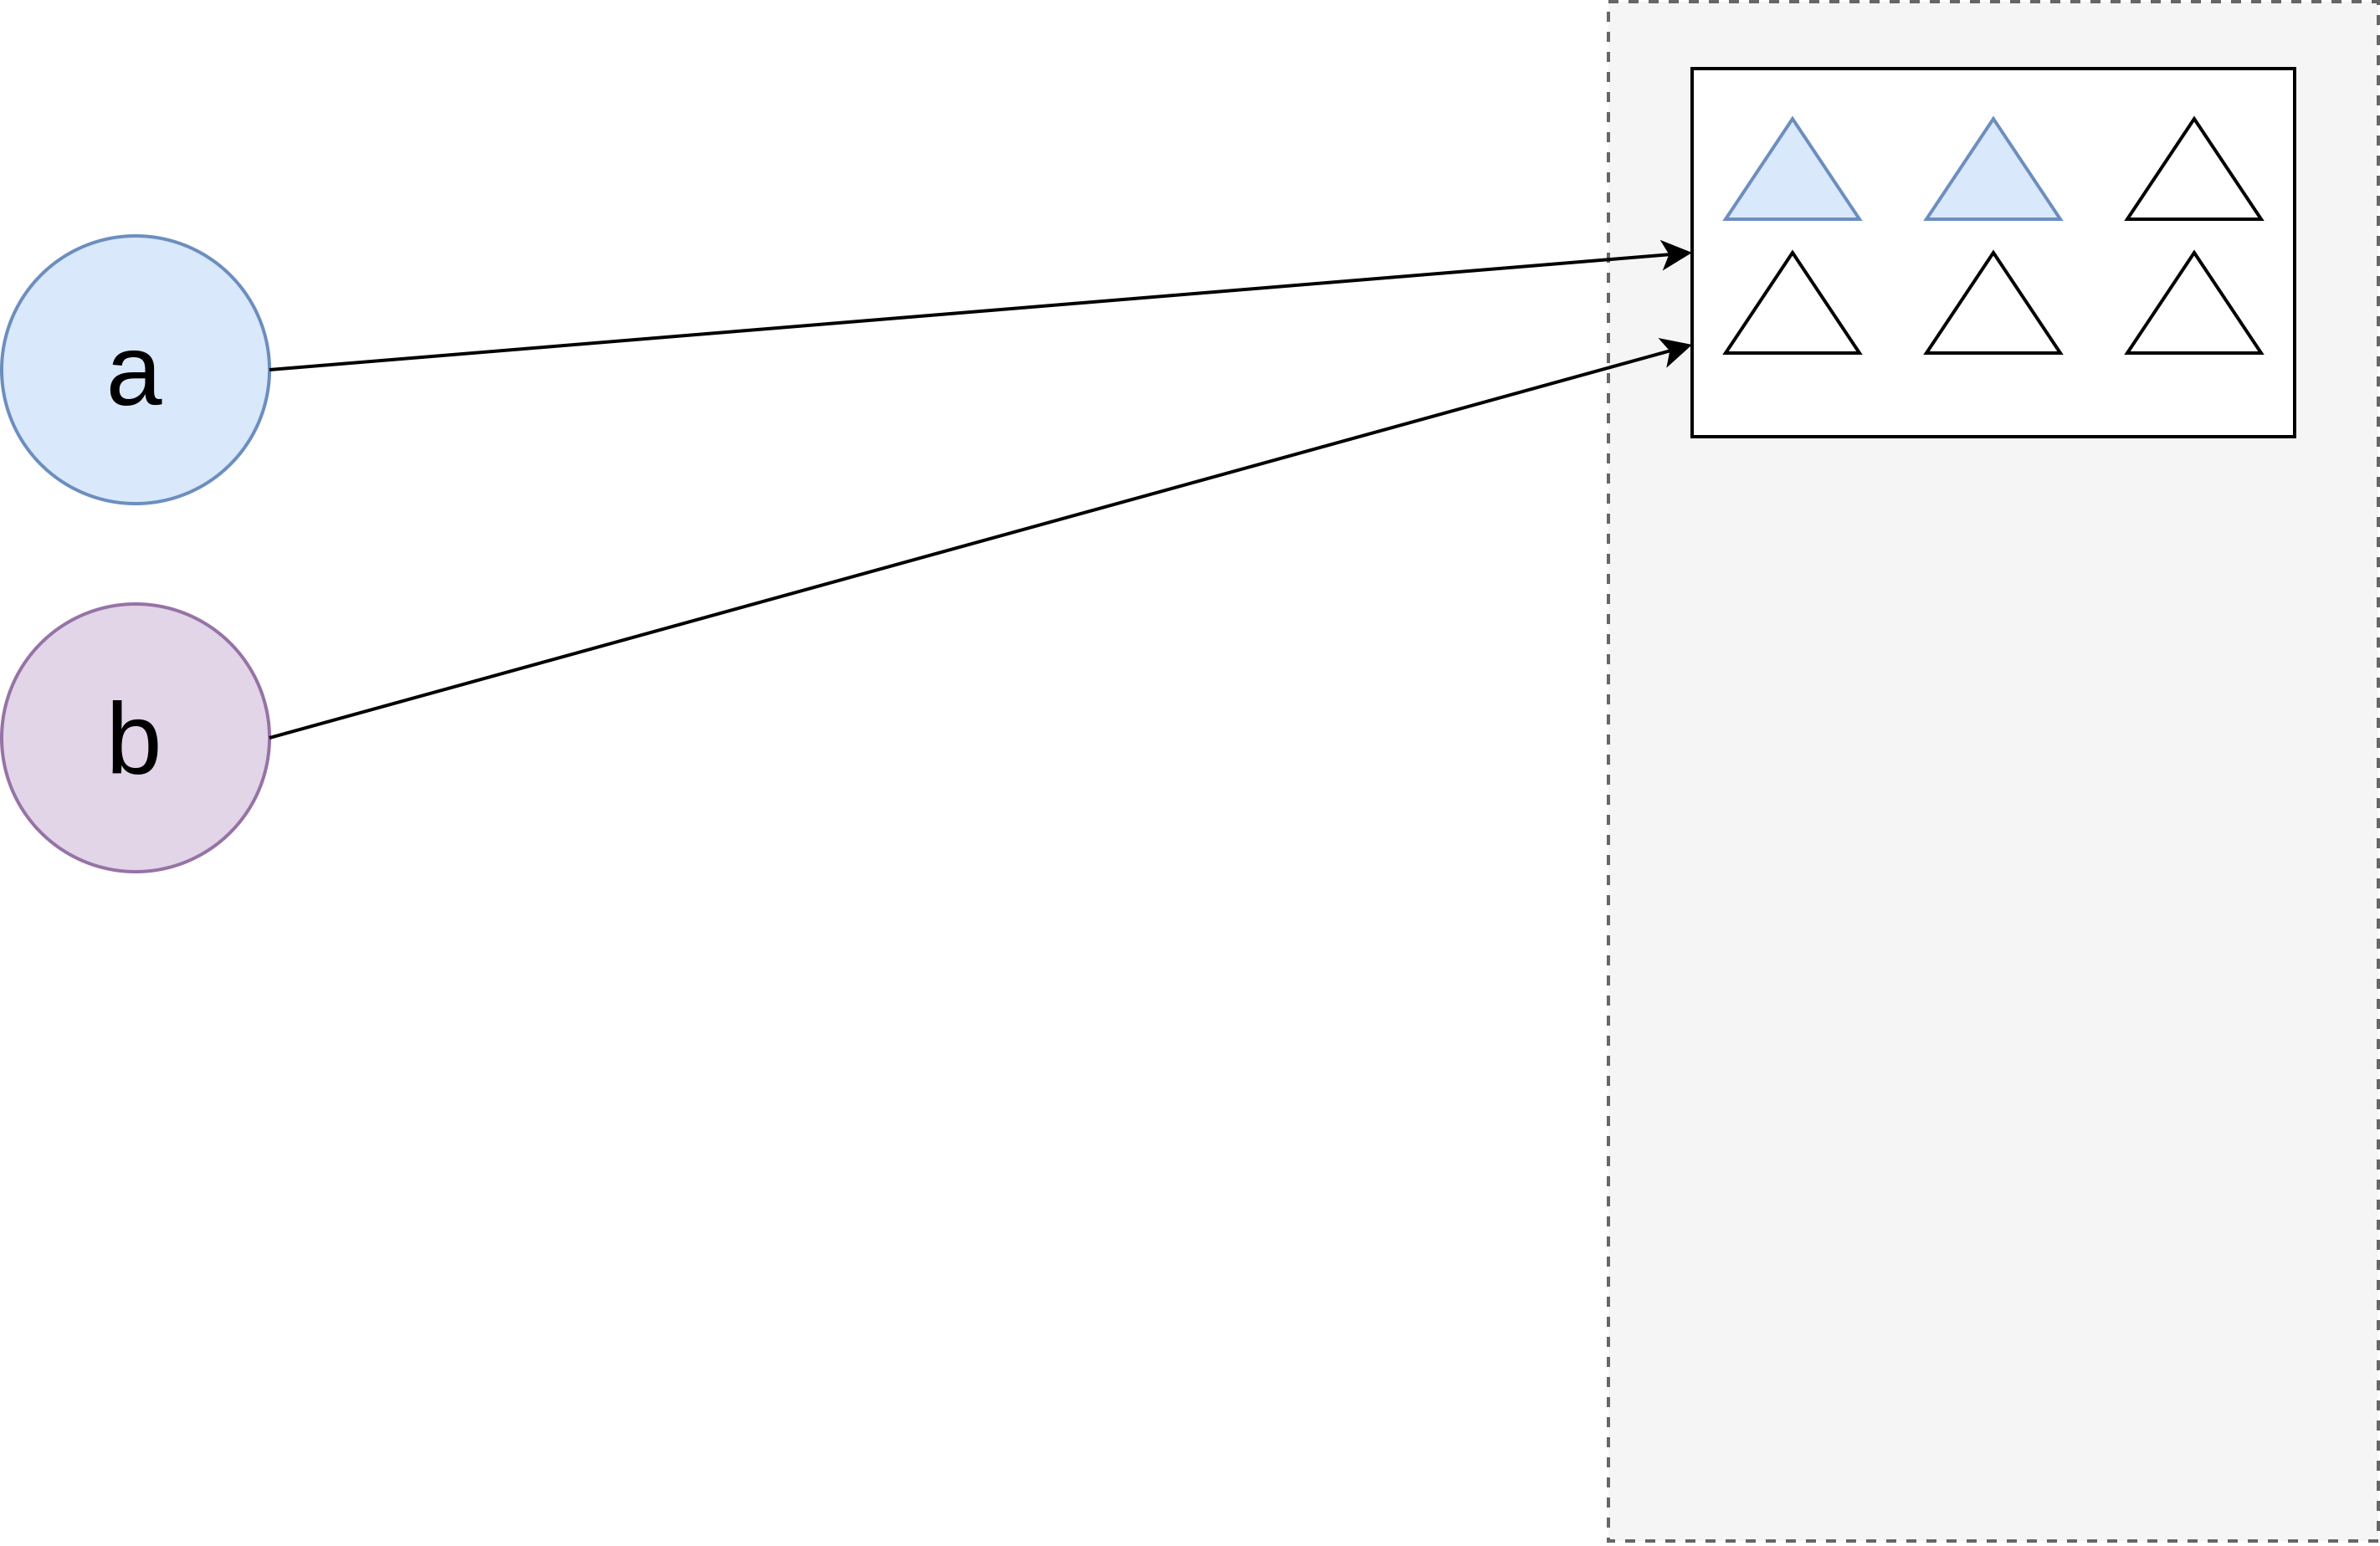
\includegraphics[height=0.7\textheight,keepaspectratio]{images/arr1.png}
        \end{figure}
        
        \framebreak
        
        \begin{figure}
            \centering
            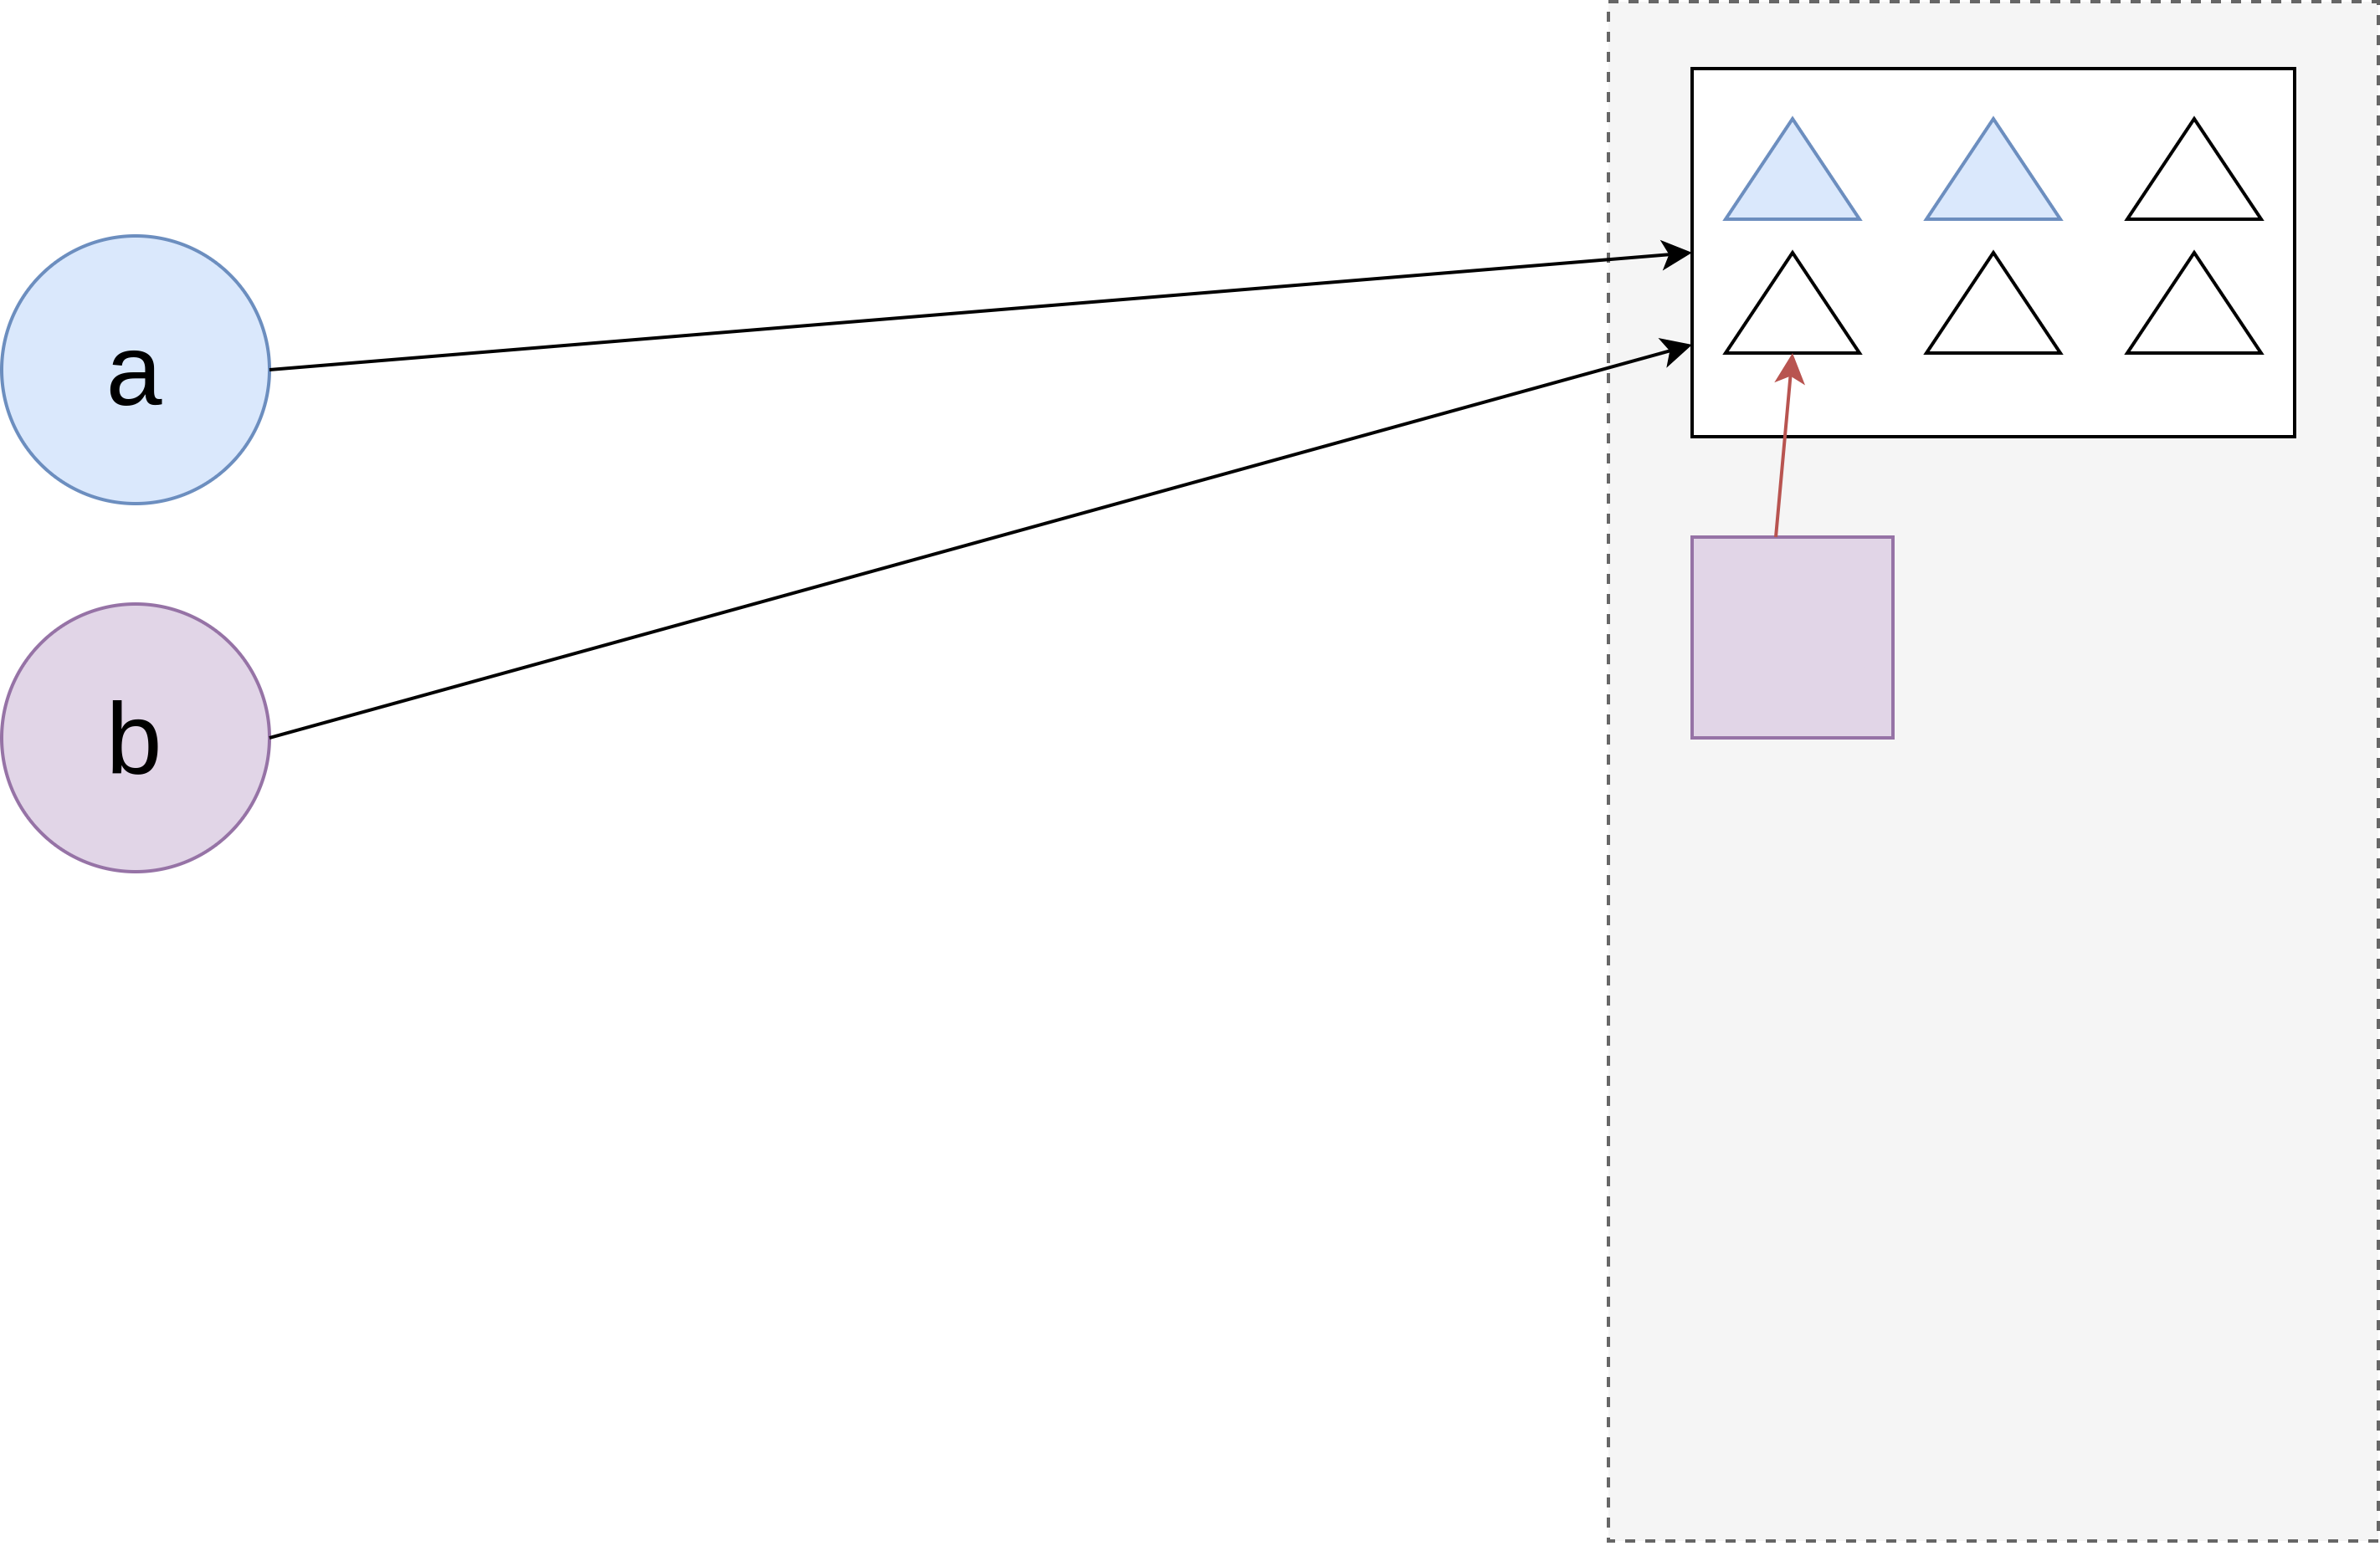
\includegraphics[height=0.7\textheight,keepaspectratio]{images/arr2.png}
        \end{figure}
        
        \framebreak
        
        \begin{itemize}
            \item Дошло је до грешке приликом извршавања кода
            \item Систем типова је то морао да спречи!
            \item Могућа решења:
            \begin{itemize}
                \item обавезно копирање низа (имутабилност)
                \item инваријантност у односу на Т
            \end{itemize}
        \end{itemize}
        
        \framebreak
        
        \begin{figure}
            \centering
            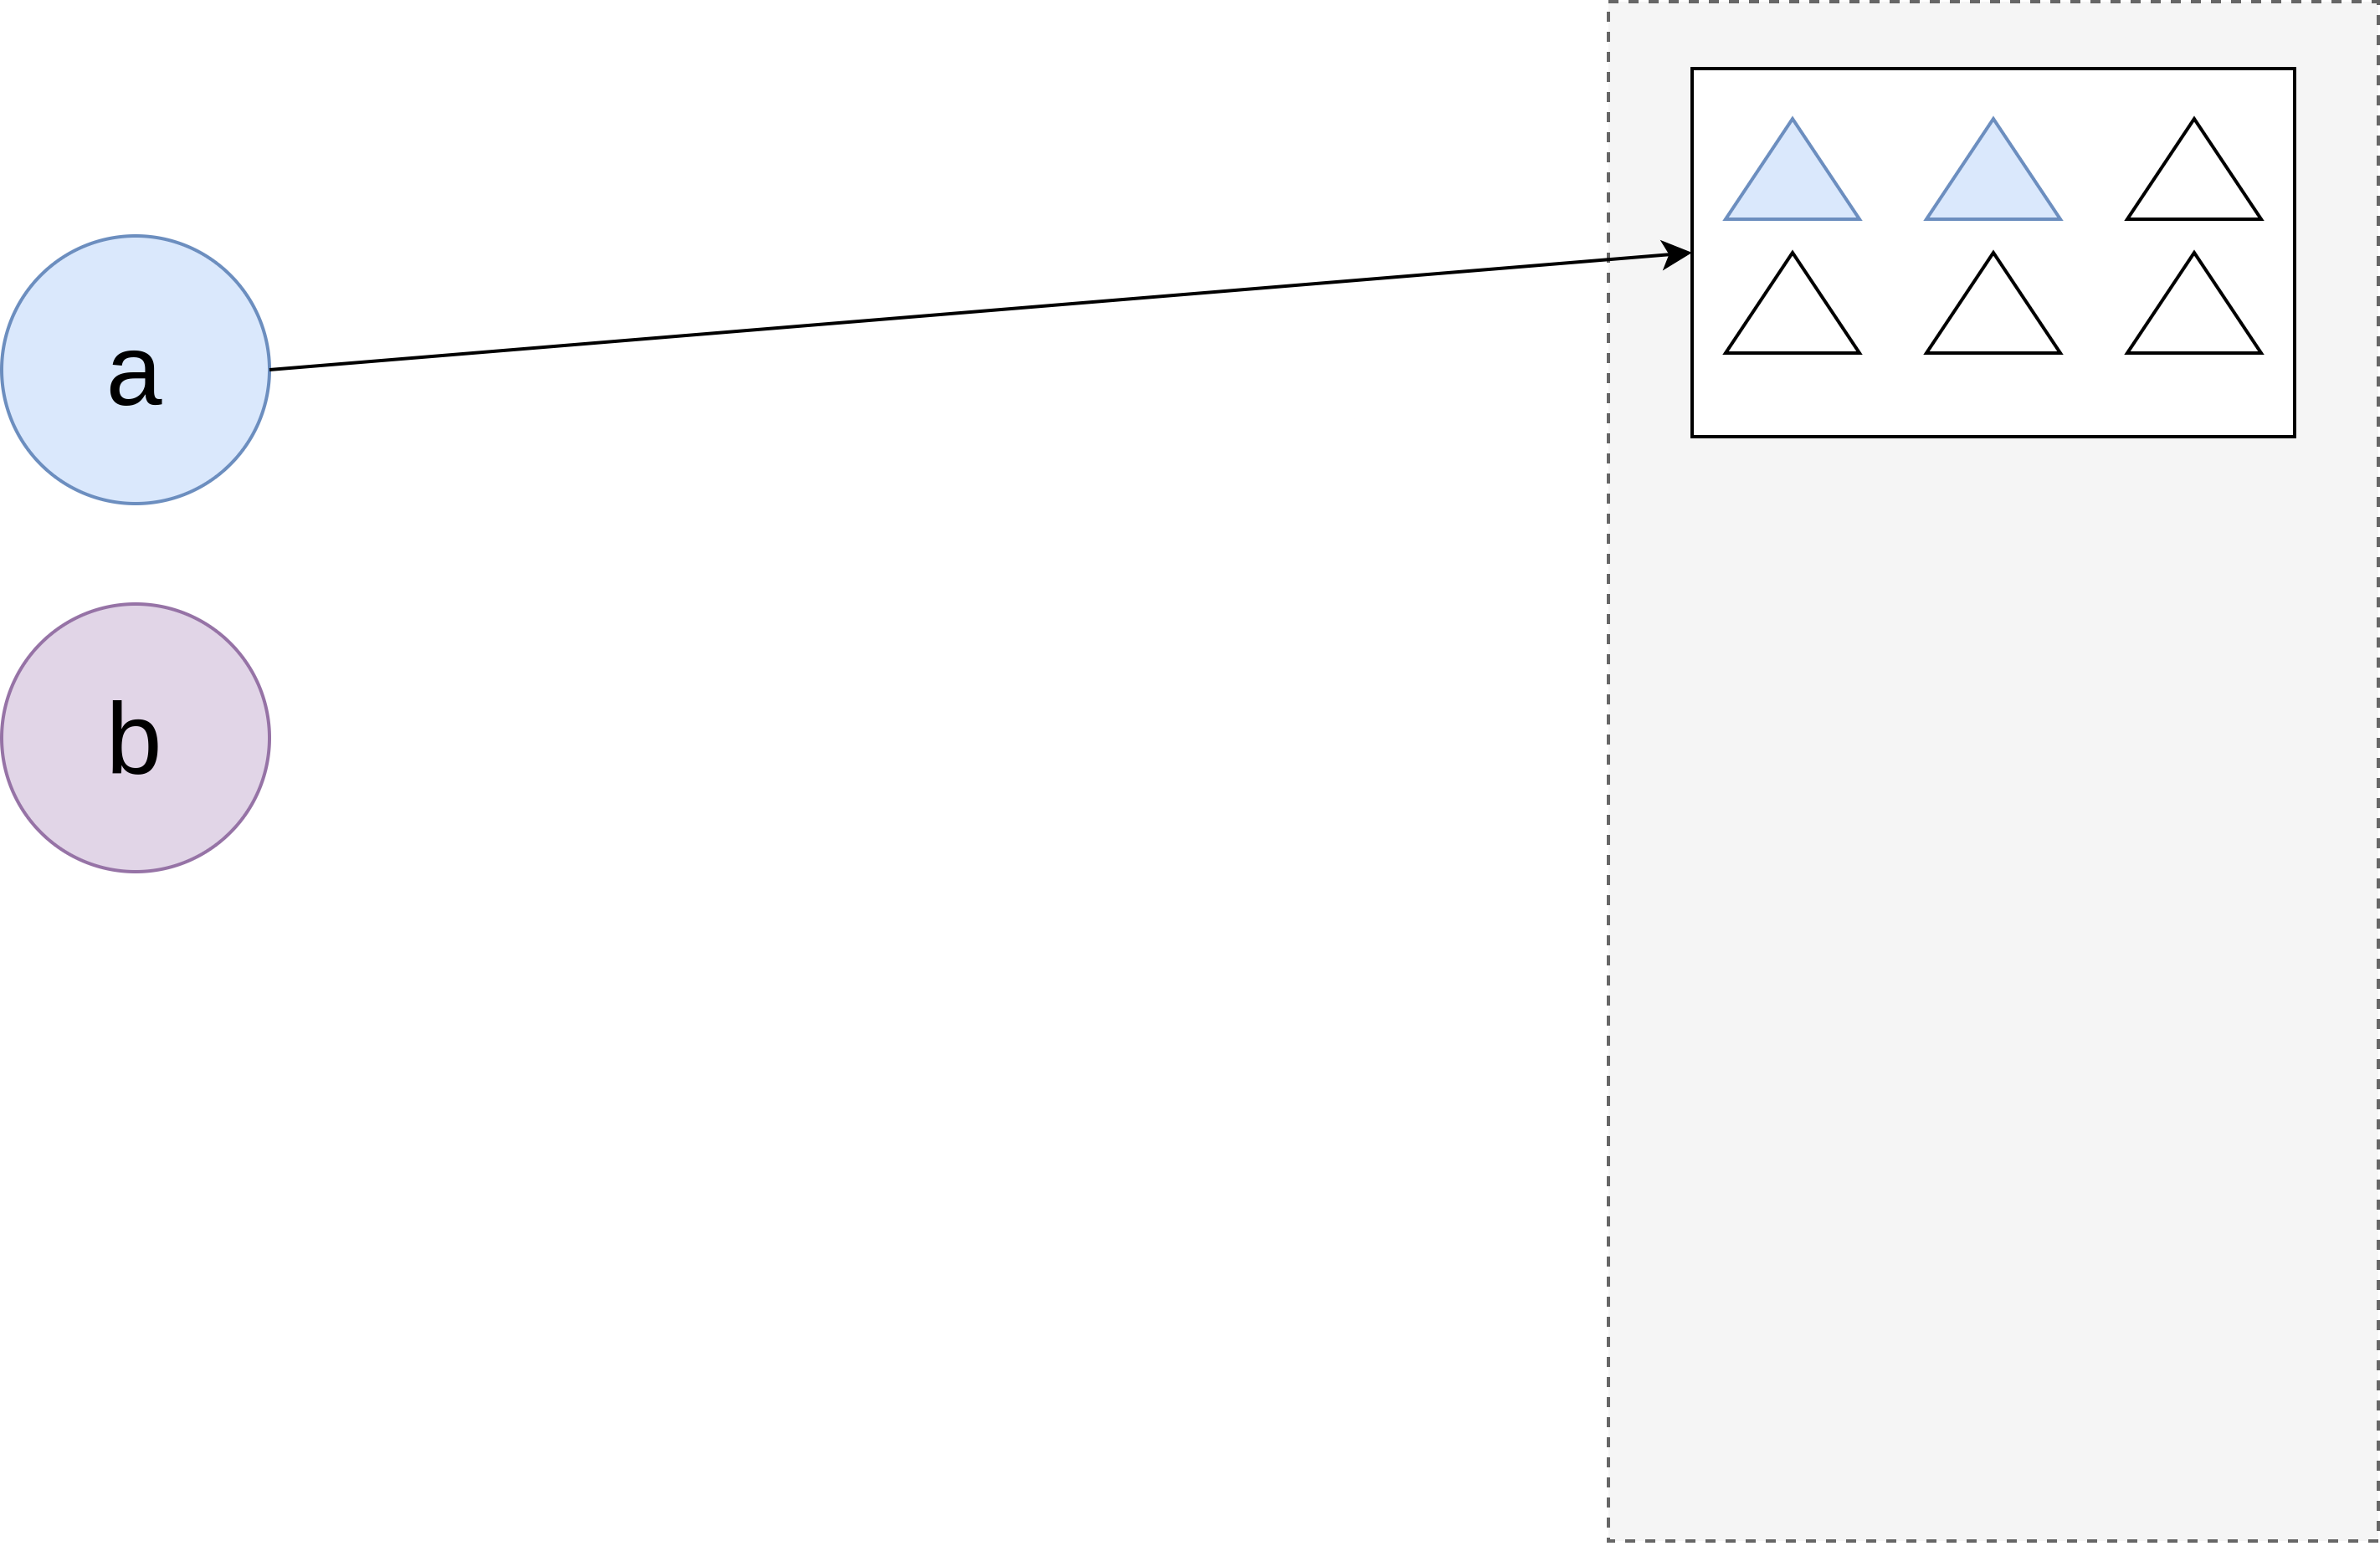
\includegraphics[height=0.7\textheight,keepaspectratio]{images/arr0.png}
        \end{figure}
        
        \framebreak
        
        \begin{figure}
            \centering
            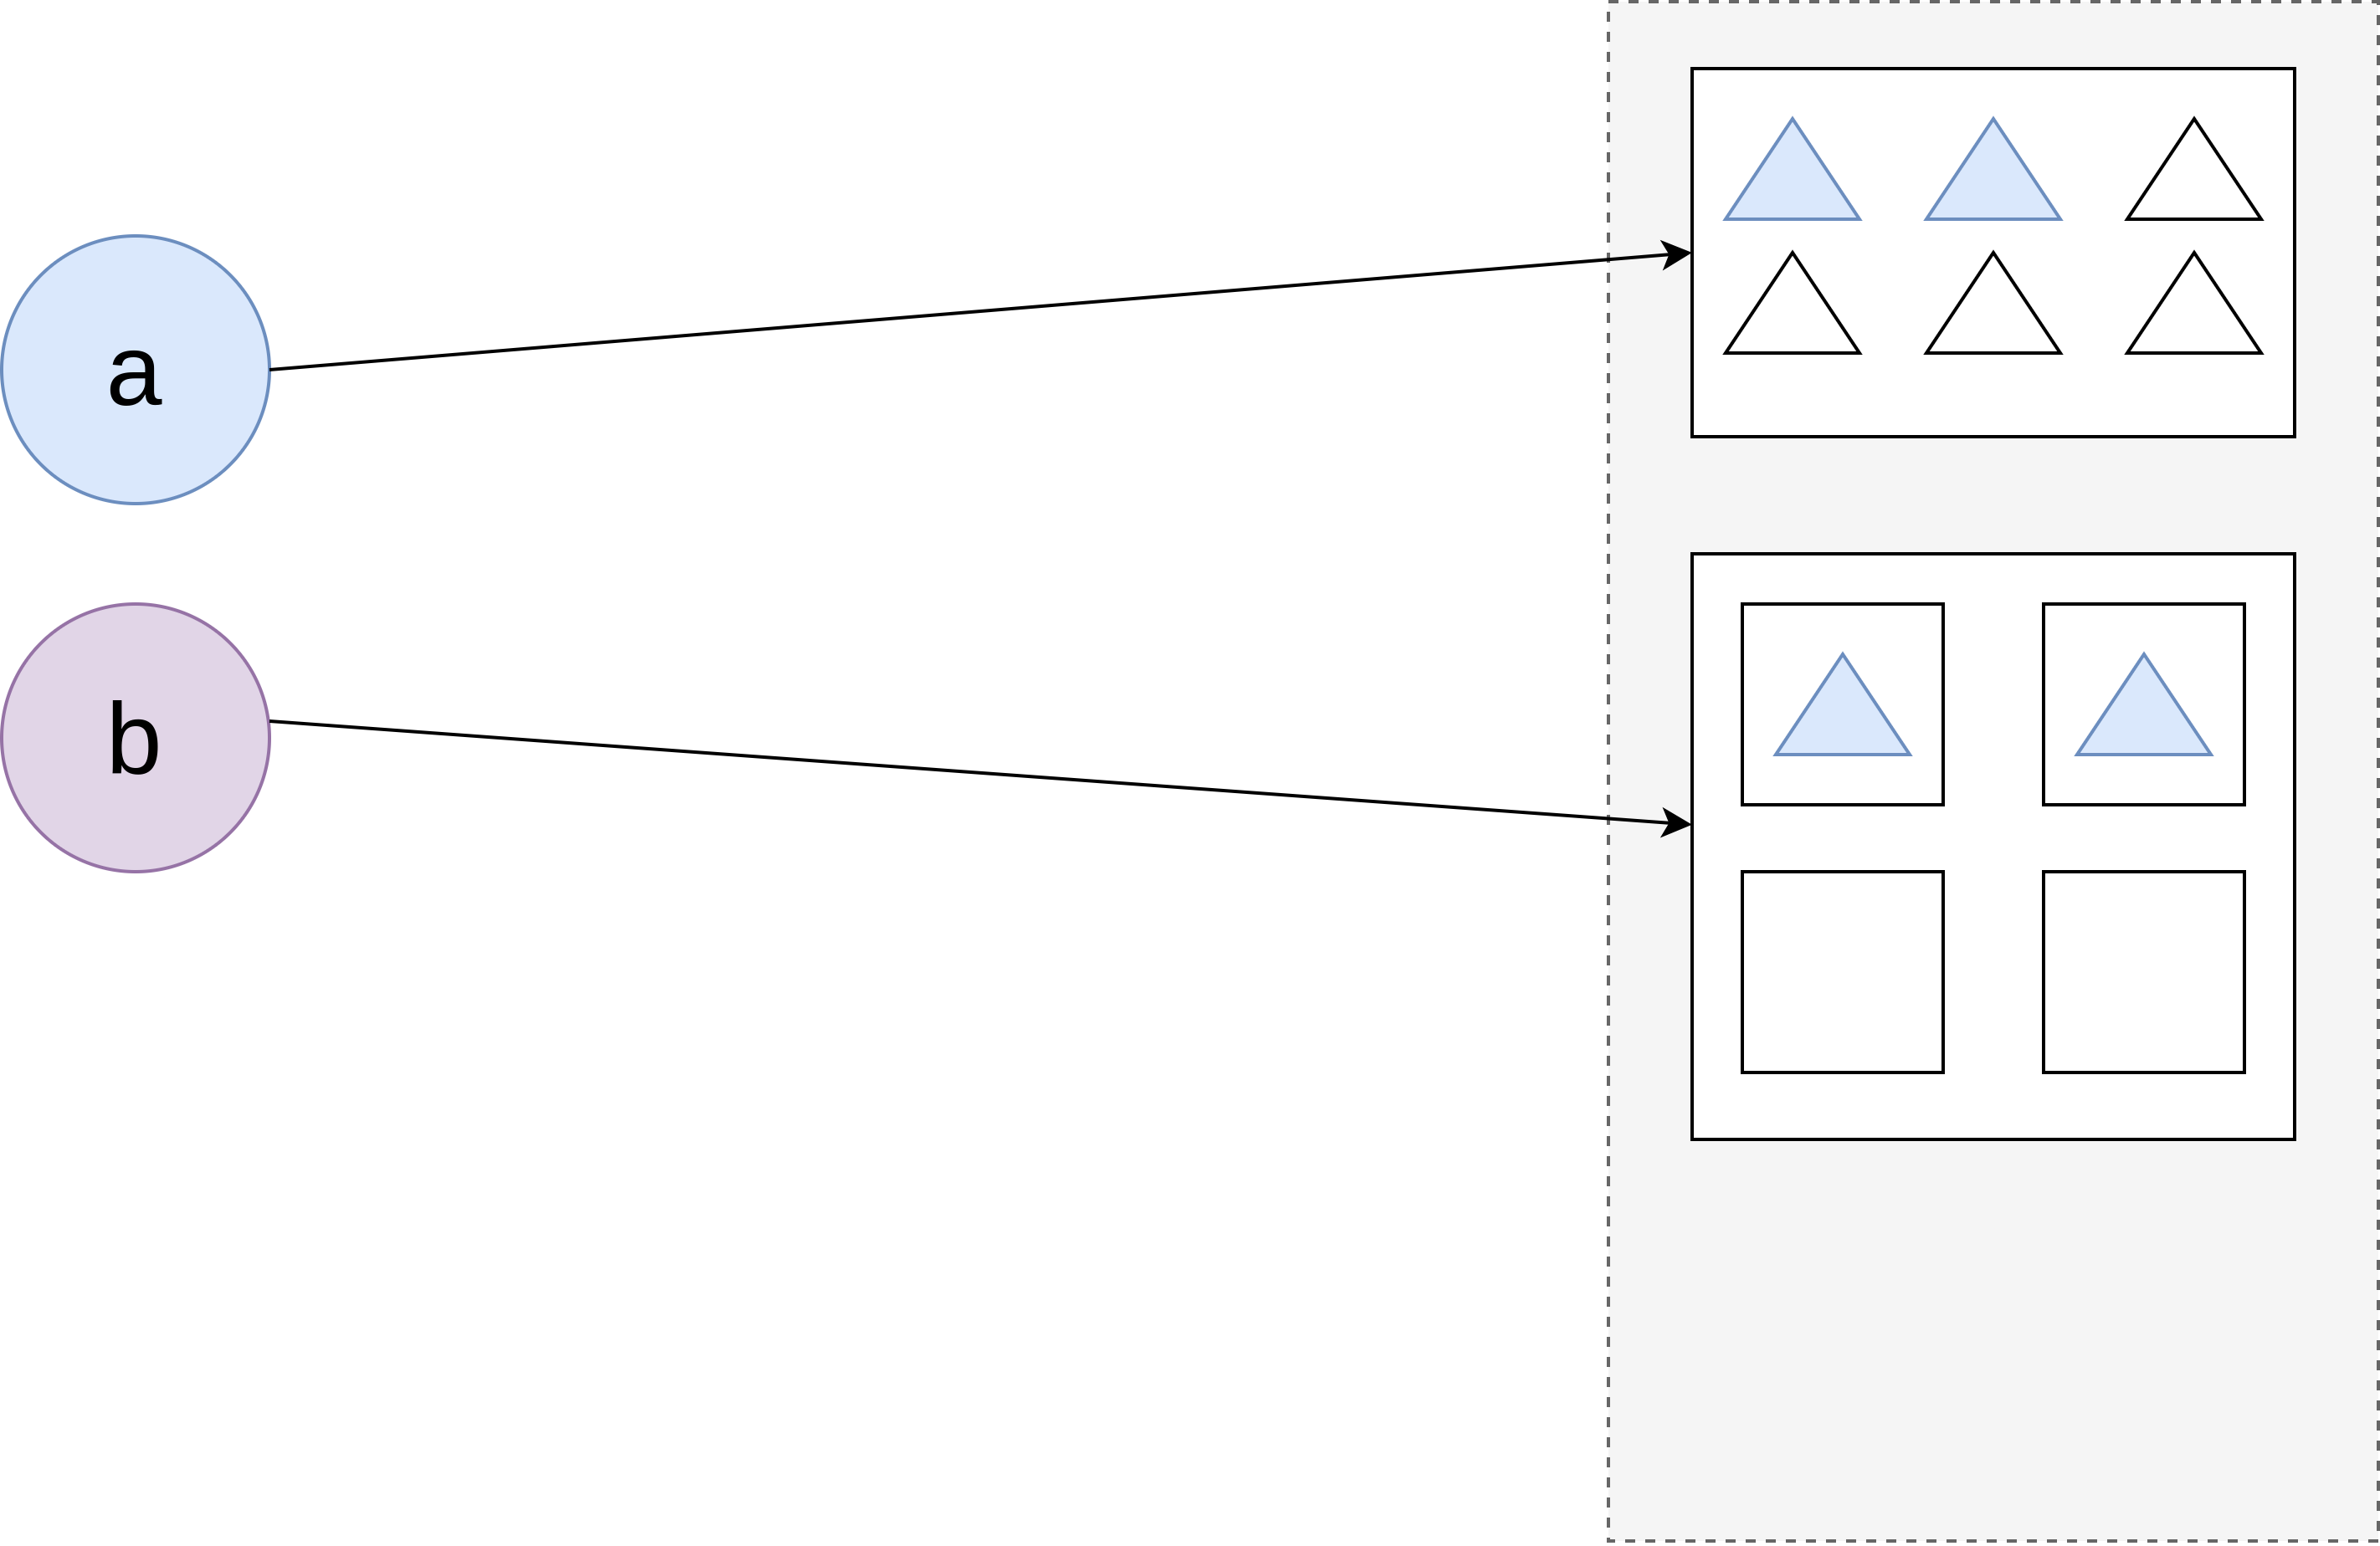
\includegraphics[height=0.7\textheight,keepaspectratio]{images/arr11.png}
        \end{figure}
        
        \framebreak
        
        \begin{figure}
            \centering
            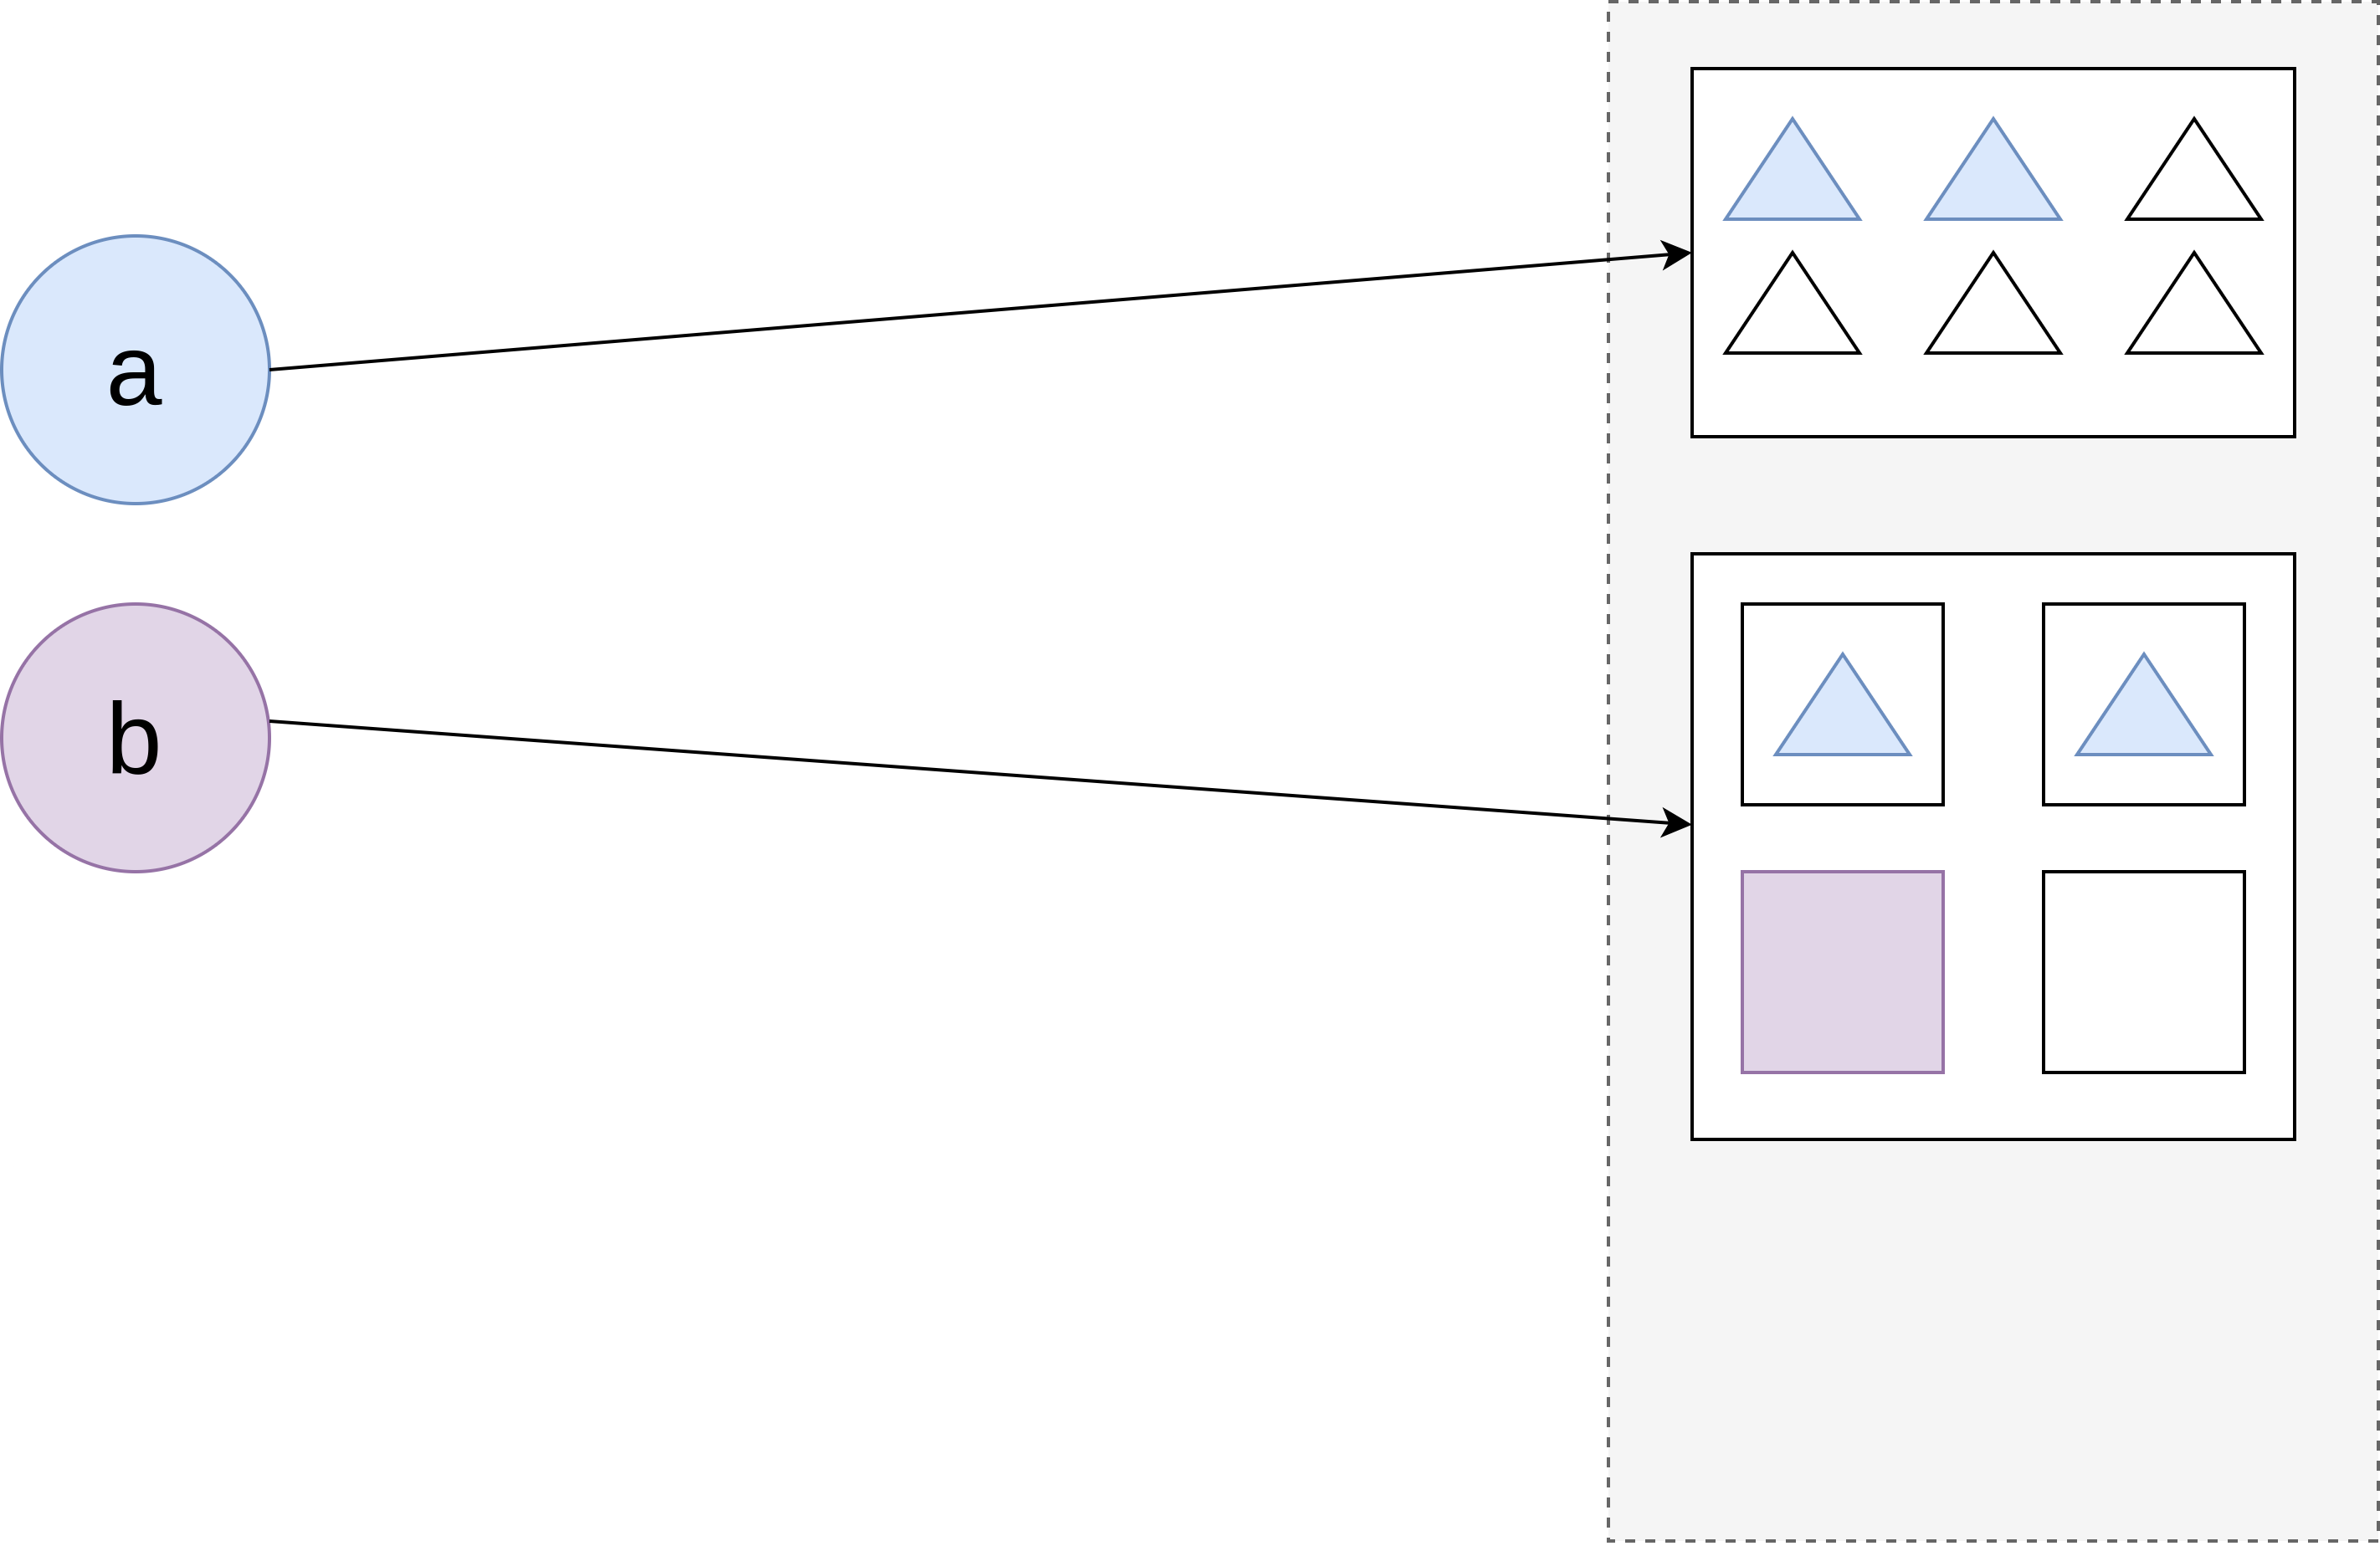
\includegraphics[height=0.7\textheight,keepaspectratio]{images/arr21.png}
        \end{figure}
    \end{frame}

    \begin{frame}{Структуре}
        \begin{itemize}
            \item Структура садржи именоване вредности (поља) чији тип може бити произвољан тип, укључујући и саму структуру из дефиниције (рекурзија је дозвољена)
            \item Које услове би требало да задовољи структура B како би важило B <= A?
            \item Проблем: мутабилност
            \begin{itemize}
                \item мутабилне структуре такође морају да буду инваријантне у односу на типове поља
                \item имутабилне структуре могу да буду варијантне
            \end{itemize}
            \item Потребно је обратити пажњу на називе поља и њихове типове
            \item Мишљења о томе како би ту пажњу требало обратити су подељена
        \end{itemize}
    \end{frame}

    \begin{frame}{Номинални системи типова}
        \textit{У номиналном систему типова, релације између сложених типова су задате приликом конструкције типова употребом ознака типова.}
    \end{frame}

    \begin{frame}{Структурални системи типова}
        \textit{У структуралном систему типова, релације између сложених типова се одређују приликом употребе типа, поређењем садржаја очекиваног и употребљеног типа.}
    \end{frame}

    \begin{frame}[allowframebreaks]{Структуре (наставак)}
        \begin{itemize}
            \item Интуиција: уколико је вредност B могуће сачувати у a: A уколико важи B <= A, да ли је правило могуће генерализовати и применити на поља структуре?
            \item Структуре су коваријантне у односу на тип појединачних поља
            \begin{itemize}
                \item поредак важи искључиво за иста поља (поља истог имена)
            \end{itemize}
            \item Иста општа правила важе и у номиналним и у структуралним системима типова
            \item Различит је начин на који се провера спроводи
        \end{itemize}

        \framebreak

        \begin{itemize}
            \item У номиналним системима типова, приликом конструкције типова се проверава да ли поља задовољавају релације у складу са осталим релацијама подтипа које је корисник задао
            \item У структуралним системима типова, приликом употребе типа у одређеном контексту се проверава да ли поља задовољавају релације у складу са релацијом између доступног и траженог типа која би требало да буде задовољена
            \item У пракси, системи типова често комбинују елементе оба приступа
        \end{itemize}
    \end{frame}

    \begin{frame}[allowframebreaks]{Функције}
        \begin{itemize}
            \item Тип функције је сложени тип који се састоји од типа параметера и типа повратне вредности
            \item Не треба мешати тип функције и тип повратне вредности функције!
            \item У језицима у којима функције представљају грађане првог реда, функције је могуће чувати у променљивама и вратити као тип израза
            \item Како можемо да дефинишемо релацију поретка?
            \item Да ли је тип функције боље посматрати и описивати номиналним или структуралним приступом?
        \end{itemize}

        \framebreak

        \begin{itemize}
            \item Интуиција: враћање вредности је једнако додели, типови функција су коваријантни у односу на тип повратне вредности
            \item Да ли на исти начин можемо да посматрамо и типове аргумената?
            \item Може ли интуиција да нас превари?
        \end{itemize}

        \framebreak

        \begin{itemize}
            \item Прослеђивање аргумената (конкретне вредности које се додељују параметрима) приликом позива фунцкије је такође једнако додели вредности
            \item Нека су A и B типови функција, а a и b променљиве
            \item Нека су типови свих параметара B подтипови параметара A
            \item Покушајмо да B доделимо у a и извршимо позив функције
        \end{itemize}

        \framebreak

        \begin{itemize}
            \item Интуиција (други покушај): како би спречили прослеђивање типа са којим функција не може да ради, неопходно је да аргументи подтипа функције буду у >= релацији у односу на аргументе надтипа функције
            \item Важи правило које је супротно од коваријантности
        \end{itemize}
    \end{frame}

    \begin{frame}{Контраваријантност типова}
    \textit{Сложени тип \begin{math}{A\mathord{<}T\mathord{>}}\end{math} је контраваријантан у односу на тип параметра \begin{math}T\end{math} уколико важи \begin{math}{A\mathord{<}X\mathord{>} \leq A\mathord{<}Y\mathord{>}}\end{math} за \begin{math}X \geq Y\end{math}}
    \end{frame}

    \begin{frame}{Функције (други покушај)}
        ..
    \end{frame}

    \begin{frame}{Генерички типови}
        \begin{itemize}
            \item До сада смо баратали искучиво са унапред познатим типовима
            \item Релација подтипа нам је давала одређену слободу да не морамо да знамо све детаље о коришћеним типовима
            \item Генеричко програмирање омогућава опис алгоритама који раде над типовима који су накнадно дефинисани
            \item Најчешћа примена: опште структуре података морају да омогуће складиштење свих корисничких типова, уз правило да се у инстанци генеричке колекције не мешају типови који нису компатибилни
            \begin{itemize}
                \item због чега релација подскупа није употребљива за ову проверу?
            \end{itemize}
        \end{itemize}
    \end{frame}

    \begin{frame}{Конструкција типова (наставак)}
        \begin{itemize}
            \item Уводи се ниво индирекције у конструкцији типова
            \item Дефиниција типа креира апстрактни тип
            \item Конструктор генеричког типа садржи параметре типова
            \item Корисник дефинише ограничења над параметрима (у виду релације подтипа)
            \item Додатно: корисник дефинише варијантност у односу на тип параметра
            \item Сви до сада наведени сложени типови могу да буду генерички типови!
        \end{itemize}
    \end{frame}

    \begin{frame}[allowframebreaks]{Унификација типова}
        \begin{itemize}
            \item Приликом креирања конкретног типа из апстрактног, корисник може да проследи произвољан тип
            \item Потребно је проверити да ли типови задовољавају ограничења која задаје апстрактни тип
            \item Додатно: потребно је доделити конкретне типове параметара
        \end{itemize}

        \framebreak

        \begin{itemize}
            \item Уколико систем типова не подржава релацију подтипа, поступак је једнак решавању система једначина
            \item Уколико је систем одређен, унификација је успешна
            \item Уколико је систем неодређен или немогућ, унификација је неуспешна
        \end{itemize}

        \framebreak

        \begin{itemize}
            \item Систем типова дефинише под којим условима је могуће унификовати два типа
            \begin{itemize}
                \item подсетник: номинални и структурални системи различито посматрају једнакост типова и релацију подтипа
                \item додатни подсетник: бабе и жабе
            \end{itemize}
            \item Опште правило:
            \begin{itemize}
                \item два проста типа је могуће унификовати уколико су једнаки
                \item два сложена типа је могуће унификовати уколико су једнаки и уколико је могуће унификовати све типове од којих се састоје
            \end{itemize}
            \item Поступак се примењује док не остану искључиво једначине познатих простих типова и параметара и простих типова
            \item Методом замене решавамо зависности између параметара
        \end{itemize}
    \end{frame}
    
    \begin{frame}{Одређен систем једначина}
        \begin{figure}
            \centering
            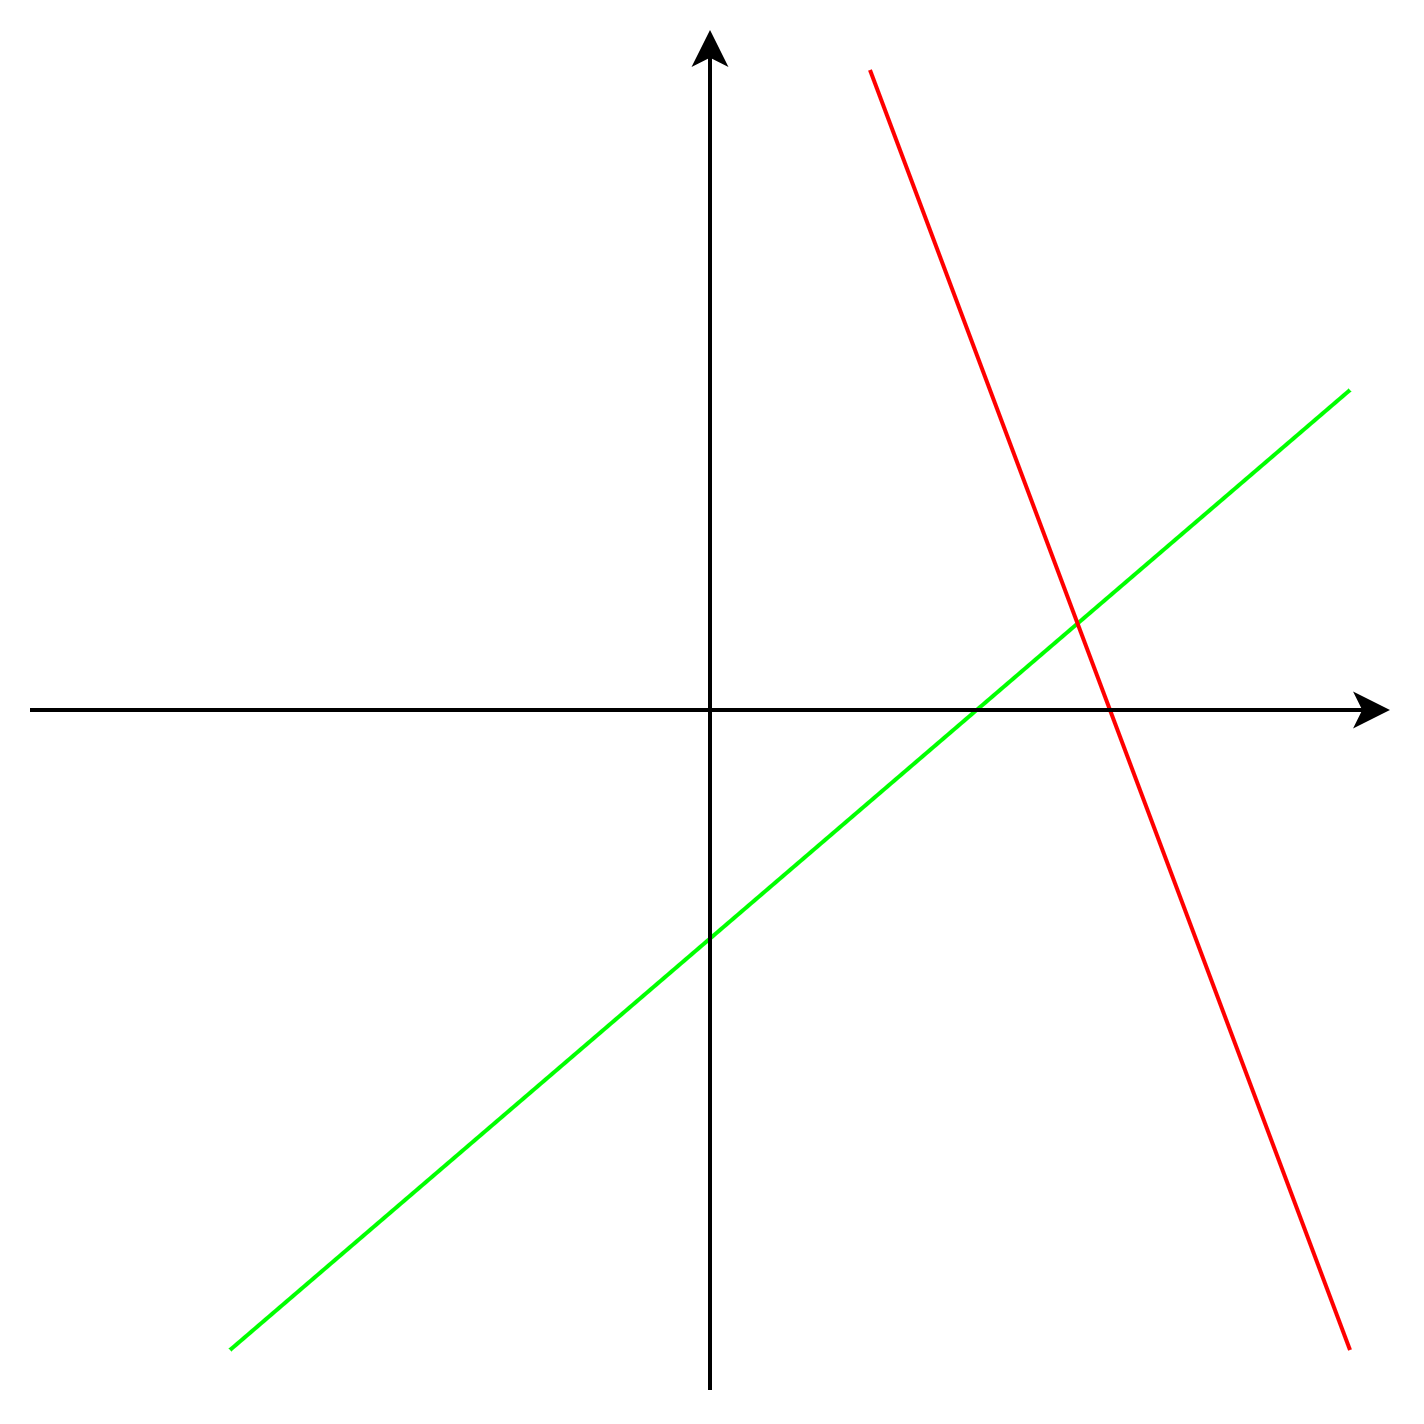
\includegraphics[width=\textwidth,height=0.8\textheight,keepaspectratio]{images/moguc_jed.png}
        \end{figure}
    \end{frame}
    
   \begin{frame}{Немогућ систем једначина}
        \begin{figure}
            \centering
            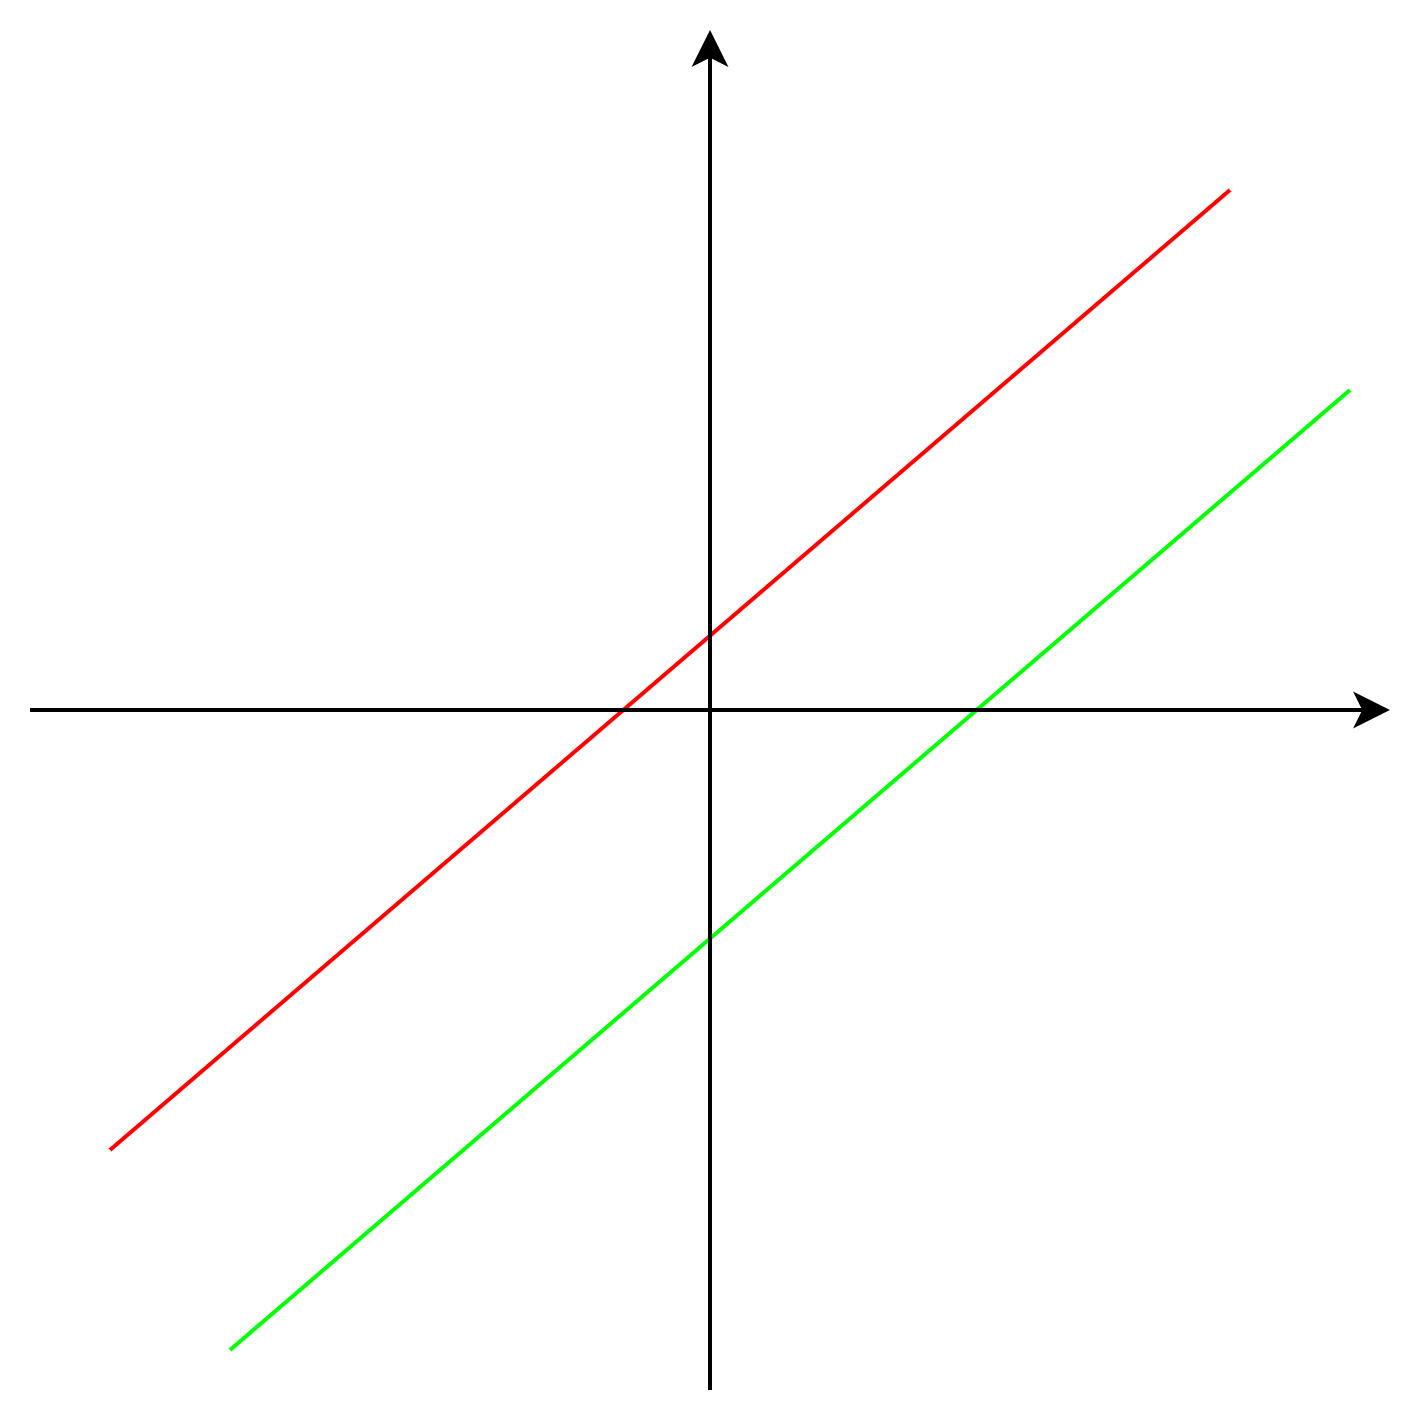
\includegraphics[width=\textwidth,height=0.8\textheight,keepaspectratio]{images/nemoguc_jed.png}
        \end{figure}
    \end{frame}
    
    \begin{frame}{Неодређен систем једначина}
        \begin{figure}
            \centering
            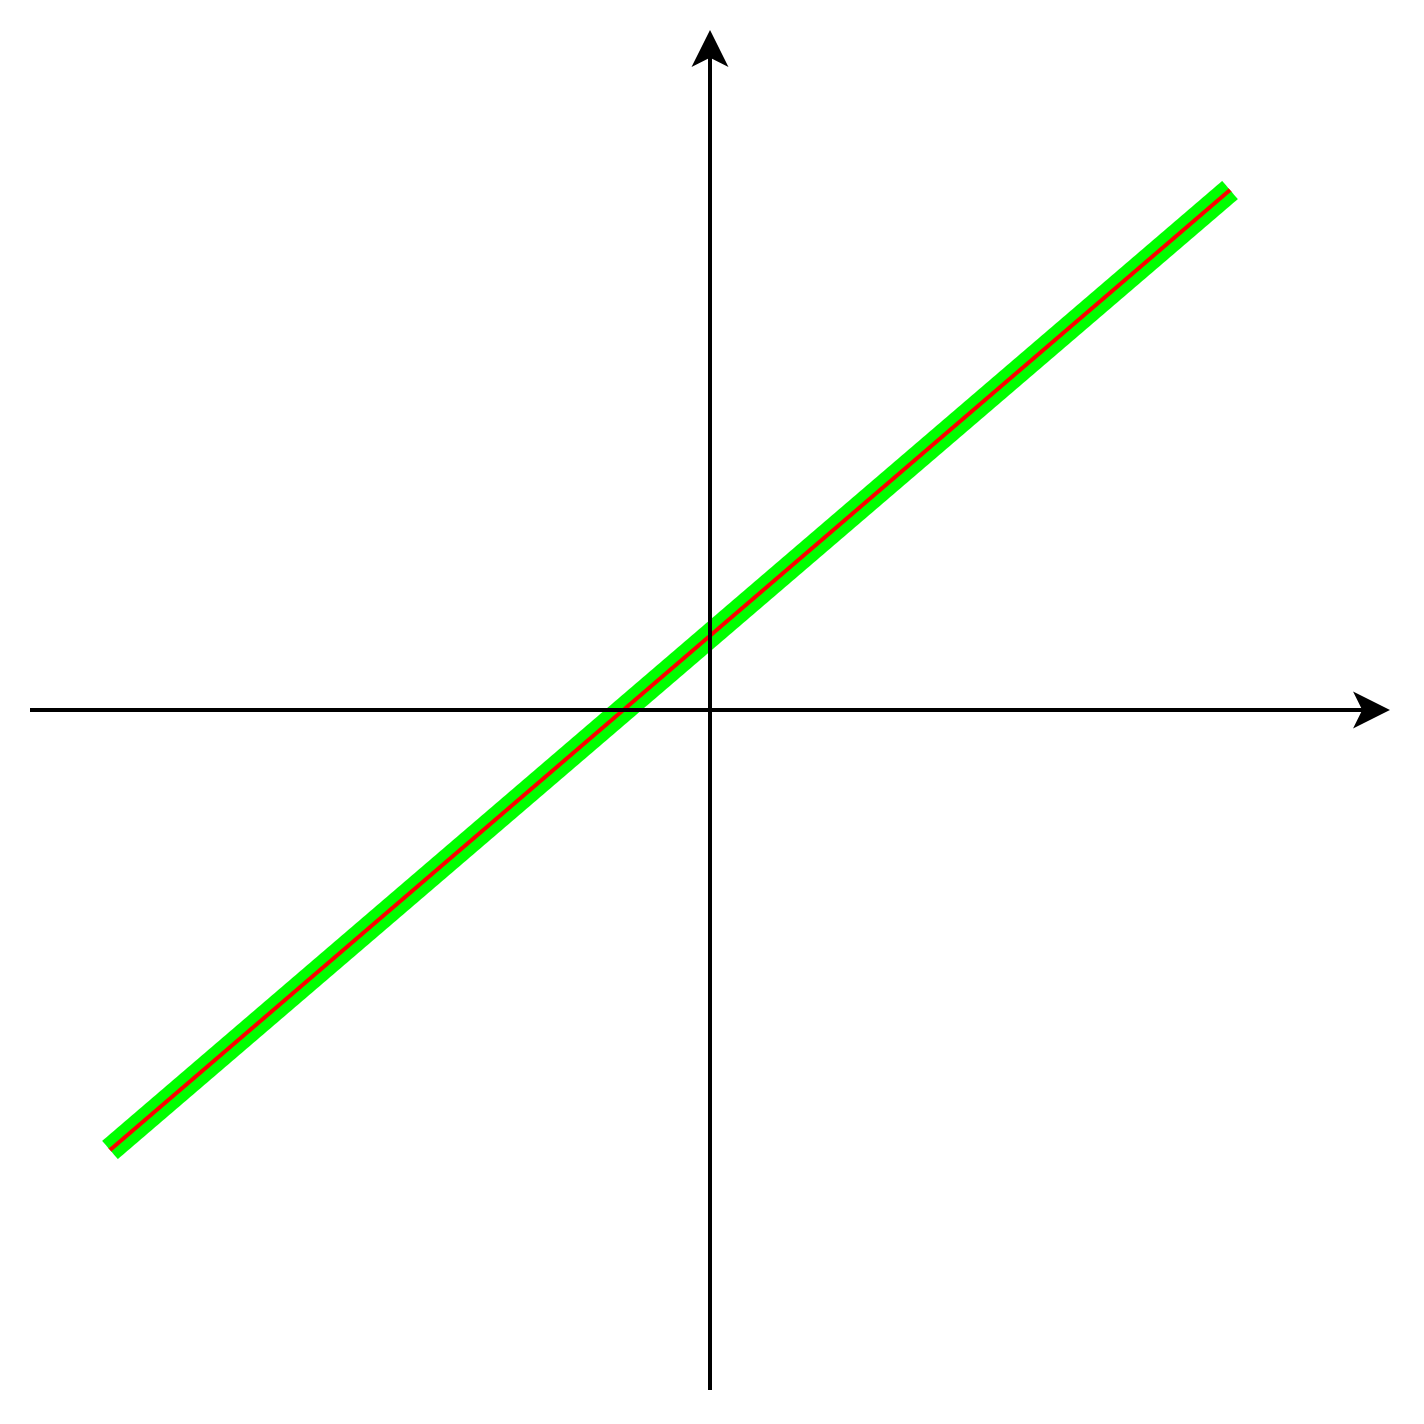
\includegraphics[width=\textwidth,height=0.8\textheight,keepaspectratio]{images/neodredjen_jed.png}
        \end{figure}
    \end{frame}
    
    \begin{frame}[allowframebreaks]{Унификација типова (поступак)}
    \begin{math}
A,B, C
\newline
List\mathord{<}T\mathord{>}
\newline
Map\mathord{<}K, V\mathord{>}
\newline
func: (a: T1, b: T2, c: List\mathord{<}T1\mathord{>}, d: List\mathord{<}T2\mathord{>}) \to Map\mathord{<}T1, T2\mathord{>}
\newline
\newline
a = A
\newline
b = B
\newline
c = List\mathord{<}A\mathord{>}
\newline
d = List\mathord{<}B\mathord{>}
\newline
\newline
x = func(a, b, c, d)
\newline
type(x) = ? 
\end{math}
        \framebreak
        
        \begin{math}
A = T1
\newline
B = T2
\newline
List\mathord{<}A\mathord{>} = List\mathord{<}T1\mathord{>}
\newline
List\mathord{<}B\mathord{>} = List\mathord{<}T2\mathord{>}
        \end{math}
        
        \framebreak
        
        \begin{math}
T1 = A
\newline
T2 = B
\newline
\newline
List = List
\newline
A = T1
\newline
List = List
\newline
B = T2
        \end{math}
        
        \framebreak
        
        \begin{math}
T1 = A
\newline
T2 = B
\newline
\newline
\text{Систем је одређен, унификација је успешна!}
\end{math}

\framebreak

\begin{math}
A,B, C
\newline
List\mathord{<}T\mathord{>}
\newline
Map\mathord{<}K, V\mathord{>}
\newline
func: (a: T1, b: T2, c: List\mathord{<}T1\mathord{>}, d: List\mathord{<}T2\mathord{>}) \to Map\mathord{<}T1, T2\mathord{>}
\newline
\newline
a = A
\newline
b = B
\newline
c = List\mathord{<}A\mathord{>}
\newline
d = List\mathord{<}A\mathord{>}
\newline
\newline
x = func(a, b, c, d)
\newline
type(x) = ? 
\end{math}
        \framebreak
        
        \begin{math}
A = T1
\newline
B = T2
\newline
List\mathord{<}A\mathord{>} = List\mathord{<}T1\mathord{>}
\newline
List\mathord{<}A\mathord{>} = List\mathord{<}T2\mathord{>}
        \end{math}
        
        \framebreak
        
        \begin{math}
T1 = A
\newline
T2 = B
\newline
\newline
List = List
\newline
A = T1
\newline
List = List
\newline
A = T2
        \end{math}
        
        \framebreak
        
        \begin{math}
T1 = A
\newline
T2 = B, T2 = A
\newline
\newline
\text{Систем је немогућ, унификација је неуспешна!}
        \end{math}
        
\framebreak
        
        \begin{math}
A,B, C
\newline
List\mathord{<}T\mathord{>}
\newline
Map\mathord{<}K, V\mathord{>}
\newline
func: (a: T1, b: T2, c: List\mathord{<}T1\mathord{>}, d: List\mathord{<}T2\mathord{>}) \to Map\mathord{<}T1, T2\mathord{>}
\newline
\newline
a = A
\newline
b = B
\newline
c = List\mathord{<}A\mathord{>}
\newline
d = Map\mathord{<}A, B\mathord{>}
\newline
\newline
x = func(a, b, c, d)
\newline
type(x) = ? 
\end{math}
        \framebreak
        
        \begin{math}
A = T1
\newline
B = T2
\newline
List\mathord{<}A\mathord{>} = List\mathord{<}T1\mathord{>}
\newline
Map\mathord{<}A, B\mathord{>} = List\mathord{<}T2\mathord{>}
        \end{math}
        
        \framebreak
        
        \begin{math}
T1 = A
\newline
T2 = B
\newline
\newline
List = List
\newline
A = T1
\newline
Map = List
\newline
\newline
\text{Унификција два различита сложена типа није могућа!}
        \end{math}
    \end{frame}

    \begin{frame}{Унификација и релација подтипа}
        \begin{itemize}
            \item Уколико систем типова подржава релацију подтипа, поступак унификације је једнак решавању система неједначина
            \item Решење има доњу и горњу границу
            \item Исправна су сва решења која су у интервалу!
            \item У пракси, бира се доња или горња граница јер резултат унификације мора да буде јединствено решење
        \end{itemize}
    \end{frame}
    
    \begin{frame}{Системи неједначина}
        \begin{figure}
            \centering
            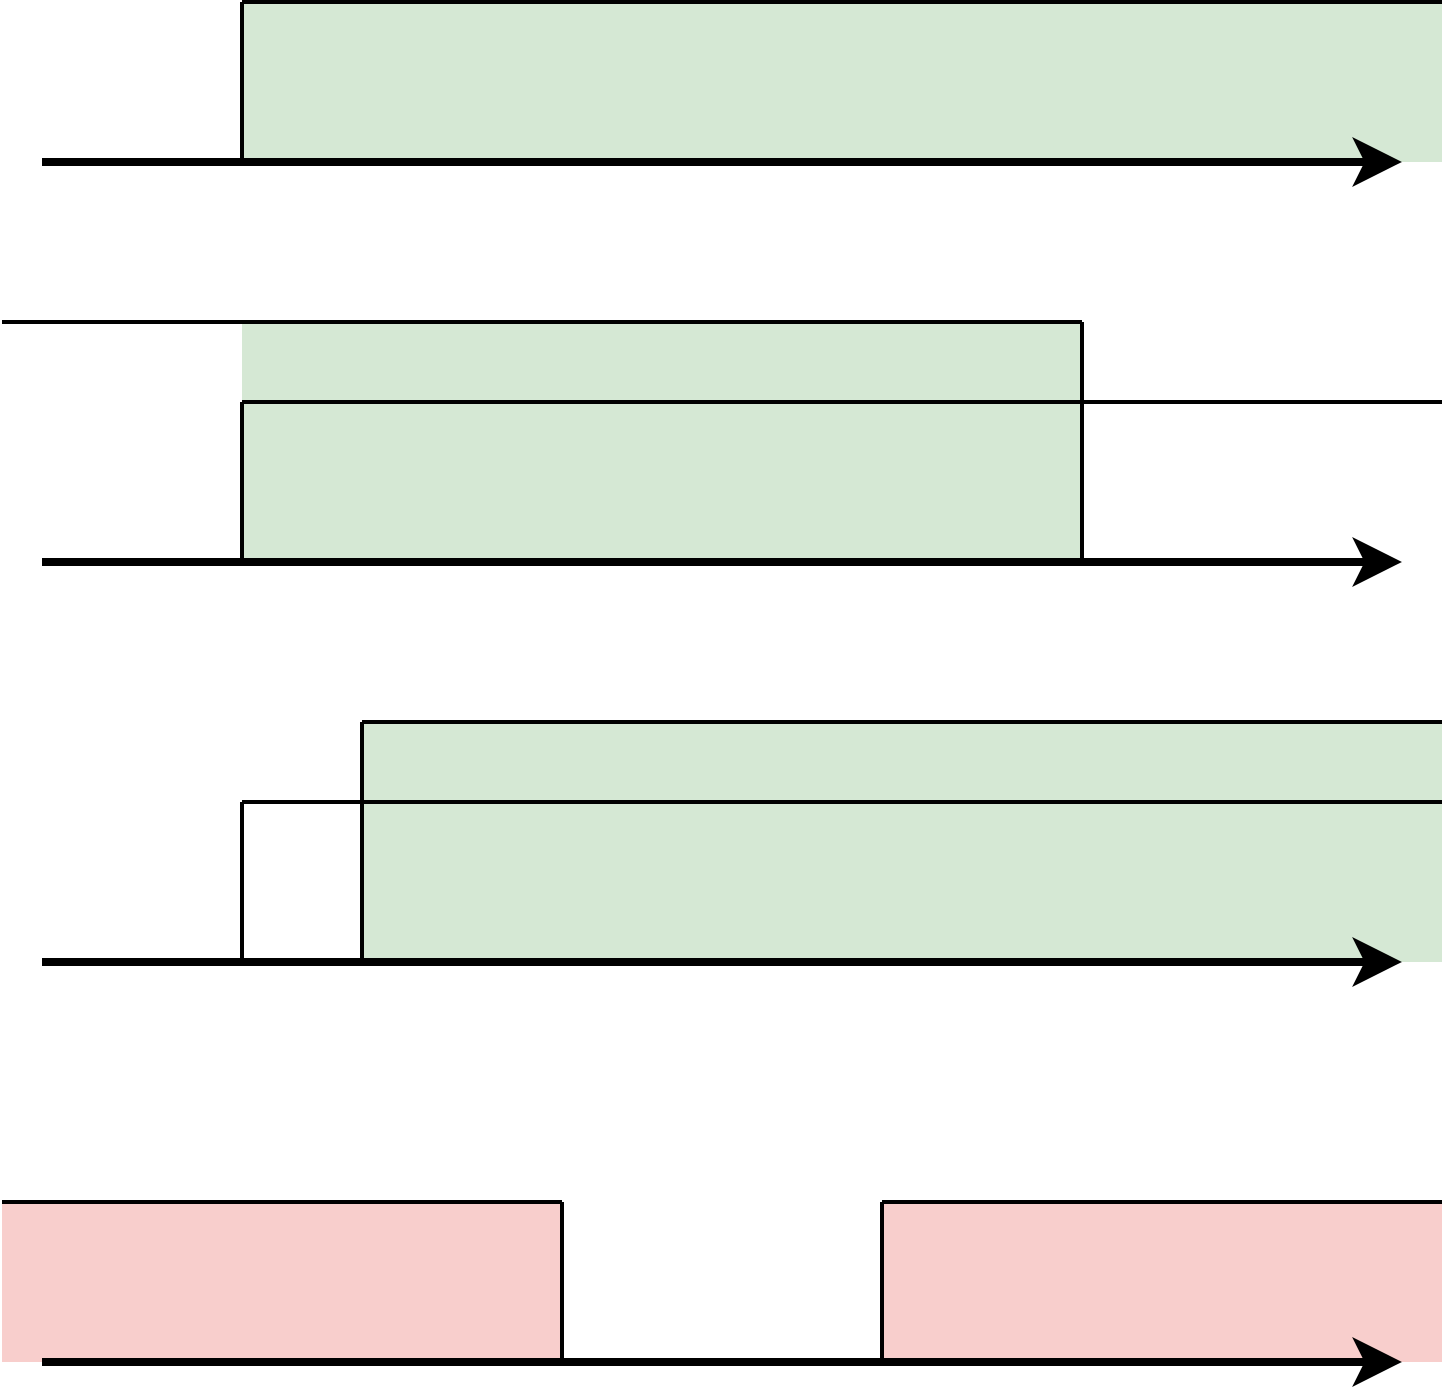
\includegraphics[width=\textwidth,height=0.8\textheight,keepaspectratio]{images/nejed_int.png}
        \end{figure}
    \end{frame}

    \begin{frame}[allowframebreaks]{Унификација типова (наставак)}
        \begin{itemize}
            \item Поступак можемо да посматрамо као генерализовану верзију претходног поступка
            \item Општа правила:
            \begin{itemize}
                \item два проста типа је могуће унификовати уколико A <= B
                \item два сложена типа је могуће унификовати уколиок A <= B и уколико је могуће унификовати све типове од којих се састоје
            \end{itemize}
            \item Додатно: решење постоји уколико је интервал правило одређен
            \item Правила за свођење израза који садрже сложене типове у изразе који садрже просте типове и параметре су приблжно иста
            \item Додатно: потребно је обратити пажњу на варијатност типова у односу на одређени параметар јер утиче на смер релације подтипа!
        \end{itemize}
    \end{frame}
    
    \begin{frame}[allowframebreaks]{Закључак}
        \begin{itemize}
            \item Као покушај налажења заједничког језика разумљивог и рачуанрима и људима, настали су виши програмски језици
            \item Додатна замисао је била аутоматска провера исправности програма
            \item Једнакост између очекиваног и обезбеђеног типа је била довољан услов да се спречи неисправна употреба вредности у програму
            \item Како појмови у природи показују сличност, замисао је била представити ту сличност кроз релацију подтипа
        \end{itemize}
        
        \framebreak
        
        \begin{itemize}
            \item Сложени типови су неопходни како би се описале појаве из природе, као и појаве из света рачунарства
            \item Релација подтипа код сложених типова зависи од конструктора типова и од садржаја самих типова
            \item За неке типове је природно да релација између садржаних типова директно одговара релацији између сложених типова (коваријантност), док је за одређене типове она супротна (контраваријантност)
            \item За разлику од математике, рачунарство познаје појам мутабилности
            \item Иако типови природно показују варијантност, мутабилност је често значајно ограничава
        \end{itemize}
        
        \framebreak
        
        \begin{itemize}
            \item Релација подтипа не обезбеђује довољну флексибилност за типове попут листа и мапа
            \item Генерички типови омогућавају да корисник при инстанцирању типа зада прецизнија ограничења типа
            \item Код генеричких типова, потребно је обавити поступак унификације како би одредили вредности непознатих параметара
            \item Уколико систем типова подржава само једнакост типова, поступак је једнак решавању система једначина
            \item Уколико систем типова подржава релацију, поступак је једнак решавању система неједначина
        \end{itemize}
    \end{frame}
    
    \begin{frame}[allowframebreaks]{Литература}
        \begin{itemize}
            \item Type Checking (Part 1), Keith Schwarz \url{https://web.stanford.edu/class/archive/cs/cs143/cs143.1128/lectures/09/Slides09.pdf}
            \item Type Checking (Part 2), Keith Schwarz \url{https://web.stanford.edu/class/archive/cs/cs143/cs143.1128/lectures/10/Slides10.pdf}
            \item Everything You Always Wanted to Know About Type Inference - And a Little Bit More, Robert Griesemer \url{https://go.dev/blog/type-inference}
            \item Unification in Chalk (part 1), Niko Matsakis \url{https://smallcultfollowing.com/babysteps/blog/2017/03/25/unification-in-chalk-part-1/}
        \end{itemize}
        
        \framebreak
        
        \begin{itemize}
            \item Type unification rules (The Go Programming Language Specification) \url{https://tip.golang.org/ref/spec\#Type_unification_rules}
            \item Kotlin type constraints (Kotlin language specification), Marat Akhin \& Mikhail Belyaev \url{https://kotlinlang.org/spec/kotlin-type-constraints.html}
            \item Type inference (Rust Compiler Development Guide) \url{https://rustc-dev-guide.rust-lang.org/type-inference.html}
        \end{itemize}
    \end{frame}
\end{document}
